% Dokumentation für Praxisprojekt                                           %%
%% (TH Köln -Campus Gummersbach, Fak. 10)                                    %%
%%                                                                           %% %%
%% LIZENZ:                                                                   %%
%% Diese Vorlage darf nicht kommerziell verbreitet                           %%
%% werden. Eine nicht-kommerzielle Weitergabe ist                            %%
%% gestattet.                                                                %%
%%                                                                           %%
%% Von Ludger Schönfeld, M. Sc.,
%% 2014-2017                            %%
%%%%%%%%%%%%%%%%%%%%%%%%%%%%%%%%%%%%%%%%%%%%%%%%%%%%%%%%%%%%%%%%%%%%%%%%%%%%%%%
%%%%%%%%%%%%%%%%%%%%%%%%%%%%%%%%%%%%%%%%%%%%%
%% HEADER                                  %%
%%%%%%%%%%%%%%%%%%%%%%%%%%%%%%%%%%%%%%%%%%%%%
\documentclass[a4paper,12pt,oneside]{article}
% Optionen:
% - a4paper => DIN A4-Format
% - 12pt    => Schriftgröße (weitere  
%              grundlegende Fontgrößen: 10pt, 11pt)
% - oneside => Einseitiger Druck
\setlength{\parindent}{0pt}

%% Verwendete Pakete:
\usepackage[ngerman]{babel} % für die deutsche Sprache
\usepackage{caption} % Für schönere Bildunterschriften
\usepackage[T1]{fontenc} % Schriftkodierung (Für Sonderzeichen u.a.)
\usepackage[utf8]{inputenc} % Für die direkte Eingabe von Umlauten im Editor u.a.
\usepackage{fancyhdr} % Für Kopf- und Fußzeilen
\usepackage{lscape} % Für Querformat

%Mehrere Bilder auf einmal
\usepackage{subfig}
\usepackage{csquotes} % Für sprachangepasste Anführungszeichen


%% Show code in a better way
\usepackage{listings}
\usepackage{xcolor}

\definecolor{dkgreen}{rgb}{0,0.6,0}
\definecolor{gray}{rgb}{0.5,0.5,0.5}
\definecolor{mauve}{rgb}{0.58,0,0.82}

\lstset{frame=tb,
  language=Java,
  aboveskip=3mm,
  belowskip=3mm,
  showstringspaces=false,
  columns=flexible,
  basicstyle={\small\ttfamily},
  numbers=none,
  numberstyle=\tiny\color{gray},
  keywordstyle=\color{blue},
  commentstyle=\color{green},
  stringstyle=\color{purple},
  breaklines=true,
  breakatwhitespace=true,
  tabsize=3
}
%% Schriften (Beispiele)
%% Weitere LaTeX-Schriften im "LaTeX Font Catalogue"
%% unter: http://www.tug.dk/FontCatalogue/.
%% ACHTUNG: Ggf. müssen Schriften noch installiert 
%% werden!

% Serifen-Schriften:
\usepackage{lmodern} % Schriftart "Latin Modern"
%\usepackage{garamond} % Schriftart "Garamond"

%Sans Serif-Schriften:
%\usepackage[scaled]{uarial}
%\usepackage[scaled]{helvet}
%%--------------
\usepackage[normalem]{ulem} % Für das Unterstreichen von Text z.B. mit \uline{}
\usepackage[left=3cm,right=2cm,top=1.5cm,bottom=1cm,
textheight=245mm,textwidth=160mm,includeheadfoot,headsep=1cm,
footskip=1cm,headheight=14.599pt]{geometry} % Einrichtung der Seite 

\usepackage{graphicx} % Zum Laden von Graphiken
\graphicspath{ {./sources/} }

% INFO: Graphiken einbinden
%
% \includegraphics[scale=1.00]{dateiname}
%
% => Ausgabeformat: PDF-Dokument:
%    Es können die folgenden (Graphik-)formate eingebunden
%    werden: .jpg, .png, .pdf, .mps
% 
% => Ausgabeformat: DVI/PS:
%    Folgende (Graphik-)formate werden unterstützt:
%    .eps, .ps, .bmp, .pict, .pntg
\usepackage{epstopdf}

% Pakete für Tabellen
\usepackage{tabularx} % Einfache Tabellen
\usepackage{longtable} % Tabellen als Gleitobjekte (für die Aufteilung bei langen 
 %Tabellen über mehrere Seiten)
\usepackage{multirow} % Für das Verbinden von Zeilen innerhalb einer Tabelle mit
 % \multirow{anzahl}{*}{Text}

% (Zusatz-)Pakete für Formeln
\usepackage{amsmath}
\usepackage{amsthm}
\usepackage{amsfonts}

\usepackage{setspace} % Paket zum Setzen des Zeilenabstandes
% INFO: Zeilenabstand setzen:
%
% Befehle:
% - \singlespacing  => 1-zeilig (Standard)
% - \onehalfspacing => 1,5-zeilig
% - \doublespacing  => 2-zeilig 
\onehalfspacing % Zeilenabstand auf 1,5-zeilig setzen

% Farbboxen (für die Merkkästen in dieser Vorlage):
\usepackage{tcolorbox}
\tcbset{colback=white,colframe=orange,
        fonttitle=\bfseries}

\usepackage[colorlinks,pdfpagelabels,pdfstartview=FitH,
bookmarksopen=true,bookmarksnumbered=true,linkcolor=black,
plainpages=false,hypertexnames=false,citecolor=black]{hyperref} % Für Verlinkungen

%Glossary
\usepackage[xindy,acronym]{glossaries}
\makeglossaries
\addcontentsline{toc}{section}{Glossar} 

%\loadglsentries{chapters/Begriffe}
%Cite
\usepackage[style=ieee]{biblatex}
\bibliography{refs} % Entries are in the refs.bib file

%%%%%%%%%%%%%%%%%%%%%%%%%%%%%%%%%%%%%%%%%%%%%
%% DOKUMENT                                %%
%%%%%%%%%%%%%%%%%%%%%%%%%%%%%%%%%%%%%%%%%%%%%
\begin{document}
% Unbeschriftetes Vorblatt (Leere Seite)
\pagestyle{empty} % Seite ohne Kopf- und Fußzeilen
\newpage % Neue Seite
\input{leereSeite} % Ausgelagerte LaTeX-Datei (hier: leereSeite.tex) einbinden

%\newpage
% Deckblatt
\pagestyle{empty}
\begin{titlepage}
  
\includegraphics[scale=0.20]{sources/TH_Koeln_Logo}\\
  \begin{center}
    \Large
    Technische Hochschule Köln\\
    Fakultät für Informatik und Ingenieurwissenschaften\\
    \hrule\par\rule{0pt}{2cm}
    \LARGE
    \textsc{BERICHT ZUM PRAXISPROJEKT}\\
    \vspace{0.8cm}
    \huge
    MVP für eine Webanwendung zur Spielersuche\\ 
    \Large
    Eine mit Javascript entwickelte Plattform \\
    \vspace{0.8cm}
    \large
    Vorgelegt an der TH Köln Campus Gummersbach\\
    im Studiengang Wirtschaftsinformatik\\
    \vspace{0.8cm}
    ausgearbeitet von:\\
    \textsc{Timo Kalker} 11127585\\
    \textsc{Carlo Menjivar} 11117929\\
    \vspace{1cm}
    \begin{tabular}{ll} % Einfache Tabelle ohne Rahmen, mit 2 Spalten erzeugen
      \textbf{Erster Prüfer:}  & Prof. Dr. Birgit Bertelsmeier \\
    \end{tabular}
    \vspace{0.5cm}
    \\Gummersbach, im Januar 2022
  \end{center}
\end{titlepage}

%\newpage
%\begin{abstract}
%  Platz für das deutsche Abstract... %TODO
%\end{abstract}

\newpage

% Inhaltsverzeichnis
\tableofcontents
\pagestyle{fancy} % Kopf- und Fußzeilen aktivieren (=> Paket "fancyhdr")

\newpage
\section*{Abbildungsverzeichnis}
\addcontentsline{toc}{section}{Abbildungsverzeichnis} % Manuellen Eintrag im Inhaltsverzeichnis erzeugen
\renewcommand{\listfigurename}{} % Name des Abbildungsverzeichnisses ändern
\thispagestyle{empty}
\listoffigures

%\newpage
%\clearpage
%\printglossaries
\section*{Glossar}%\label{Begriffe}
%%% MUSTER %%%
%\newglossaryentry{}
%{name=, description={}}

%%%%%%%%%%%%
%%% TIMO %%%
%%%%%%%%%%%%

\newglossaryentry{MVP}
{
    name=MVP,
    description={Minimum Viable Product, erste funktionsfähige Version des Produkts; dient dazu zu prüfen, ob es Sinn macht, das Produkt weiterzuentwickeln und ggf. anzupassen}
}


\newglossaryentry{Responsive Webdesign}
{
    name=Responsive Webdesign,
    description={Die Webseite wird so aufgebaut, dass sie auf möglichst vielen Endgeräten mit verschiedenen Bildschirmgrößen und Eingabemethoden (Maus, Touchscreen) skaliert wird und bedienbar ist.}
}

\newglossaryentry{DQL}
{
    name=DQL,
    description={Data Query Language, Datenabfragesprache für SQL}
}

\newglossaryentry{Tinder}
{
    name=Tinder,
    description={Datingportal, bei der Nutzer in Kontakt treten, indem sie sich bei der Kontaktsuche gegenseitig einen \enquote{like} geben}
}

\newglossaryentry{Brute-Force-Angriff}
{
    name=Brute-Force-Angriff,
    description={Versuch, ein Passwort zu knacken, indem jede mögliche Kombination nacheinander ausprobiert wird.}
}

\newglossaryentry{UI/UX}
{
    name=UI/UX,
    description={User Interface / User Experience. Benutzeroberfläche / Benutzerfreundlichkeit.} 
}

\newglossaryentry{MERN}
{
    name=MERN,
    description={Beliebter Techstack für das Web, bei dem MongoDB, ExpressJS, React und NodeJS verwendet werden}
}

\newglossaryentry{MongoDB}
{
    name=MongoDB,
    description={Beliebte Dokumentbasierte Datenbank}
}

\newglossaryentry{NodeJS}
{
    name=NodeJS,
    description={JS-Laufzeit, die es ermöglicht, JS auf dem Server auszuführen}
}

\newglossaryentry{Express}
{
    name=Express,
    description={Framework für NodeJS, welches die Entwicklung von Webanwendungen vereinfacht}
}

\newglossaryentry{React}
{
    name=React,
    description={JS UI-Framework für Webseiten}
}

\newglossaryentry{JavaScript}
{
    name=JavaScript,
    description={Beliebte Scriptsprache, die vor allem für Webseiten verwendet wird. Neben Web-Assembly die einzige Sprache, welche sich auf Klienten-Seite ausführen lässt. Nach ECMAScript standardisiert}
}

\newglossaryentry{REST-API}
{
    name=REST-API,
    description={REpresentional State Transfer; Architekturstil, der eine Schnittstelle über die Protokolloptionen POST (Create), GET (Read),  PUT/PATCH (Update) und DELETE (Delete) nach RFC-2616 ermöglicht}
}

\newglossaryentry{AWS S3}
{
    name=AWS S3,
    description={Amazon Simple Storage Service; Objektspeicher über Webschnittstelle}
}

\newglossaryentry{Multer}
{
    name=Multer,
    description={Middleware für NodeJS zum behandeln von POST-Anfragen des Typs \enquote{multipart/form-data}}
}

\newglossaryentry{Apollo}
{
    name=Apollo,
    description={Beliebte Implementation der GraphQl-Spezifikation}
}

\newglossaryentry{Mongoose}
{
    name=Mongoose,
    description={NodeJS-Paket zur Objektmodellierung von MongoDB}
}

\newglossaryentry{NoSQL}
{
    name=NoSQL,
    description={Not only SQL; Sammelbegriff für Datenbanken, die einen nicht-relationalen Ansatz verfolgen.}
}

\newglossaryentry{ORDBMS}
{
    name=,
    description={ObjektRelationales DatenBank ManagementSysten}
}

\newglossaryentry{ACID}
{
    name=ACID,
    description={Atomicity, Consistency, Isolation, Durability; häufig erwünschte Eigenschaften von Transaktionen von Datenbanken}
}

\newglossaryentry{JSON}
{
    name=JSON,
    description={JavaScipt Object Notation; Datenformat zum Austausch von Daten zwischen Anwendungen}
}

\newglossaryentry{Sharding}
{
    name=Sharding,
    description={Methode der Datenbankpartitionierung, Aufteilung der Datenbank in mehrere \enquote{Scherben}, die zusammen alle Daten verwalten}
}

\newglossaryentry{Replikatgruppe}
{
    name=Replikatgruppe,
    description={Gruppe von Datenbankprozessen, welche die selben Daten verwalten. Dadurch wird Redundanz und Hocherreichbarkeit gewahrt.}
}

\newglossaryentry{Constraint}
{
    name=Constraints,
    description={Bedingung, die eine Variable erfüllen muss, um in die Datenbank aufgenommen zu werden.}
}

\newglossaryentry{Multi-Master-Systeme}
{
    name=Multi-Master-Systeme,
    description={Datenbanksysteme, welche mehrere Prozesse ermöglichen, Schreibzugriffe durchzuführen.}
}

\newglossaryentry{Write-Ahead-Log}
{
    name=Write-Ahead-Log,
    description={Protokoll, welches vor jeder Datenänderung der PostgreSQL-Datenbank erstellt wird. Dies verringert die nötige Anzahl an Schribzugriffen und erleichtert das Erstellen und Aufspielen von Backups}
}

\newglossaryentry{Salt}
{
    name=,
    description={Wert, der dem zu hashenden Wert vor dem Hashen hinzugefügt wird, um die Wahrscheinlichkeit gleicher Eingabewerte zu verringern und damit die Informationssicherung zu erhöhen.}
}

\newglossaryentry{DDOS-Angriff}
{
    name=DDOS-Angriff,
    description={Distributed Denial Of Service Attack; Angriff eines Webdienstes durch Überlastung durch etliche Anfragen von einer Vielzahl von Geräten}
}

\newglossaryentry{DBaaS}
{
    name=DBaaS,
    description={DataBase as a Service; Datenbankinfrastruktur wird vom Anbieter aus der Cloud bezogen, statt diese selbst zu betreuen}
}

\newglossaryentry{Dev-Prod-Vergleichbarkeit}
{
    name=Dev-Prod-Vergleichbarkeit,
    description={Regel 10 der 12-Faktor-App, Entwicklungs- und Produktionsumgebung so ähnlich wie möglich halten, um die Probleme durch Inkompatibilitäten zu vermeiden}
}

\newglossaryentry{npm}
{
    name=npm,
    description={node package manager; Bibliothek und Paketmanager für Pakete der NodeJS-Runtime}
}

\newglossaryentry{RFC-7519}
{
    name=RFC-7519,
    description={Norm, auf der JSON Web Tokens basieren}
}

\newglossaryentry{JSON Web Token}
{
    name=JSON Web Token,
    description={Nach RFC-7519 genormter Zugriffsschlüssel, durch den die Identität des Nutzers einer Webseite gespeichert wird}
}

\newglossaryentry{API}
{
    name=API,
    description={Application Programming Interface; Programmierschnittstelle, durch die verschiedene Programme Daten austauschen können}
}

\newglossaryentry{Mutation}
{
    name=Mutation,
    description={Veränderung der bestehenden Daten nach GraphQl-Spezifikation, entspricht POST/PUT/PATCH/DELETE in REST-API}
}

\newglossaryentry{Angular}
{
    name=Angular,
    description={Angular ist ein Framework von Google für die Entwicklung von Mobil- und Webanwendungen. } 
}

\newglossaryentry{TypeScript}
{
    name=TypeScript,
    description={Superset von JS, wird zur Laufzeit nach JS transpiliert, bietet im Gegensatz zu JS starke Typisierung an, dadurch wird eine Quelle für Softwarefehler vermieden}
}

\newglossaryentry{ECMAScript 2015}
{
    name=ECMAScript 2015,
    description={ES2015, früher ES6; Eine Version von ECMAScript, die viele neue Funktionen bietet, JS basiert auf ECMAScript}
}

\newglossaryentry{XSS-Angriff}
{
    name=XSS-Angriff,
    description={Cross-Side-Scripting; Art der HTML-Injection, Kann auftreten, wenn Nutzereingaben mit Schadcode ungefiltert vom Server akzeptiert und ausgeführt werden}
}

\newglossaryentry{StackOverFlow}
{
    name=StackOverFlow,
    description={Beliebtes Programmierer-Forum}
}

\newglossaryentry{Github}
{
    name=Github,
    description={Beliebter Dienst zur Versionsverwaltung für Entwicklungsprojekte.}
}

\newglossaryentry{HTML-DOM}
{
    name=HTML-DOM,
    description={Das HTML-DOM ist ein Standardobjektmodell und eine Programmierschnittstelle für HTML.} 
}

\newglossaryentry{Jest}
{
    name=Jest,
    description={Beliebtes JS Testing-Framework. Stand 2022.}
}

\newglossaryentry{Cypress}
{
    name=Cypress,
    description={Cypress ist ein End-to-End-Test-Framework für die Automatisierung von Web-Tests.} 
}

\newglossaryentry{OpenBase}
{
    name=OpenBase,
    description={OpenBase hilft Entwicklern bei der Auswahl aus Millionen von Open-Source-Paketen} 
}

\newglossaryentry{Framework}
{
    name=Framework,
    description={Liefert einen Rahmen mit verschiedenen Funktionen, die für das Schreiben einer Anwendung verwendet und selektiv angepasst werden können.}
}

\newglossaryentry{atomare Tests}
{
    name=atomare Tests,
    description={Softwartests, welche in sich abgeschlossen sind und andere Tests nicht beeinflussen.}
}

\newglossaryentry{UTF-8}
{
    name=UTF-8,
    description={Weit verbreitete Kodierung für Unicode-Zeichen, sehr beliebt für Webseiten}
}

\newglossaryentry{DQL}
{
    name=DQL,
    description={Data Query Language, Datenabfragesprache für SQL}
}

%PRINTING BEGRIFFE
\textbf{ACID}\\
Atomicity, Consistency, Isolation, Durability; häufig erwünschte Eigenschaften von Transaktionen von Datenbanken.
\\\\
\textbf{atomare Tests}\\
Softwartests, welche in sich abgeschlossen sind und andere Tests nicht beeinflussen.
\\\\
\textbf{Angular}\\
Angular ist ein Framework von Google für die Entwicklung von Mobil- und Webanwendungen.
\\\\
\textbf{Apollo}\\
Beliebte Implementation der GraphQl-Spezifikation.
\\\\
\textbf{API}\\
Application Programming Interface; Programmierschnittstelle, durch die verschiedene Programme Daten austauschen können.
\\\\
\textbf{AWS S3}\\
Amazon Simple Storage Service; Objektspeicher über Webschnittstelle.
\\\\
\textbf{DQL}\\
Data Query Language, Datenabfragesprache für SQL
\\\\
\textbf{Destrukturierende Zuweisung}\\
Die destrukturierende Zuweisung ermöglicht es, Daten aus Arrays oder Objekten zu extrahieren, und zwar mit Hilfe einer Syntax, die der Konstruktion von Array- und Objekt-Literalen nachempfunden ist.
%\url{https//developer.mozilla.org/de/docs/Web/JavaScript/Reference/Operators/Destructuring_assignment}
\\\\
\textbf{MVP}\\
Minimum Viable Product, erste funktionsfähige Version des Produkts; dient dazu zu prüfen, ob es Sinn macht, das Produkt weiterzuentwickeln und ggf. anzupassen.
\\\\
\textbf{JSX}\\
Es heißt JSX und ist eine Syntaxerweiterung für JavaScript. JSX erinnert vielleicht an eine Template-Sprache, aber es verfügt über die volle Leistungsfähigkeit von JavaScript. JSX erzeugt React-"Elemente"
\\\\
\textbf{Over-Fetching}\\
Empfang von überschüssigen Daten durch eine Abfrage.
%Reference https//jwt.io/
\\\\
\textbf{undefined}\\
Eine Variable, der kein Wert zugewiesen wurde oder die überhaupt nicht deklariert wurde (nicht deklariert, existiert nicht), ist undefiniert. Eine Methode oder Anweisung gibt auch undefiniert zurück, wenn der ausgewerteten Variablen kein Wert zugewiesen wurde. Eine Funktion gibt undefiniert zurück, wenn kein Wert zurückgegeben wurde.
\\\\
\textbf{Responsive Webdesign}\\
Die Webseite wird so aufgebaut, dass sie auf möglichst vielen Endgeräten mit verschiedenen Bildschirmgrößen und Eingabemethoden (Maus, Touchscreen) skaliert wird und bedienbar ist.
\\\\
\textbf{UTF-8}\\
Weit verbreitete Kodierung für Unicode-Zeichen, sehr beliebt für Webseiten.
\\\\
\textbf{Web Token}\\
JSON-Web-Tokens sind eine dem Industriestandard RFC 7519 entsprechende Methode zur sicheren Darstellung von Forderungen zwischen zwei Parteien.
\\\\
\textbf{Tinder}\\
Datingportal, bei der Nutzer in Kontakt treten, indem sie sich bei der Kontaktsuche gegenseitig einen like geben.
\\\\
\textbf{Brute-Force-Angriff}\\
Versuch, ein Passwort zu knacken, indem jede mögliche Kombination nacheinander ausprobiert wird.
\\\\
\textbf{UI/UX}\\
User Interface / User Experience. Benutzeroberfläche / Benutzerfreundlichkeit.
\\\\
\textbf{MERN}\\
Beliebter Techstack für das Web, bei dem MongoDB, ExpressJS, React und NodeJS verwendet werden.
\\\\
\textbf{MongoDB}\\
Beliebte Dokumentbasierte Datenbank.
\\\\
\textbf{NodeJS}\\
JS-Laufzeit, die es ermöglicht, JS auf dem Server auszuführen.
\\\\
\textbf{Express}\\
Framework für NodeJS, welches die Entwicklung von Webanwendungen vereinfacht.
\\\\
\textbf{React}\\
JS UI-Framework für Webseiten.
\\\\
\textbf{JavaScript}\\
Beliebte Scriptsprache, die vor allem für Webseiten verwendet wird. Neben Web-Assembly die einzige Sprache, welche sich auf Klienten-Seite ausführen lässt. Nach ECMAScript standardisiert.
\\\\
\textbf{REST-API}\\
REpresentional State Transfer; Architekturstil, der eine Schnittstelle über die Protokolloptionen POST (Create), GET (Read),  PUT/PATCH (Update) und DELETE (Delete) nach RFC-2616 ermöglicht.
\\\\
\textbf{Multer}\\
Middleware für NodeJS zum behandeln von POST-Anfragen des Typs multipart/form-data.
\\\\
\textbf{Mongoose}\\
NodeJS-Paket zur Objektmodellierung von MongoDB.
\\\\
\textbf{NoSQL}\\
Not only SQL; Sammelbegriff für Datenbanken, die einen nicht-relationalen Ansatz verfolgen.
\\\\
\textbf{ORDBMS}\\
ObjektRelationales DatenBank ManagementSysten.
\\\\
\textbf{JSON}\\
JavaScipt Object Notation; Datenformat zum Austausch von Daten zwischen Anwendungen.
\\\\
\textbf{Sharding}\\
Methode der Datenbankpartitionierung, Aufteilung der Datenbank in mehrere Scherben die zusammen alle Daten verwalten.
\\\\
\textbf{Replikatgruppe}\\
Gruppe von Datenbankprozessen, welche die selben Daten verwalten. Dadurch wird Redundanz und Hocherreichbarkeit gewahrt.
\\\\
\textbf{Constraint}\\
Bedingung, die eine Variable erfüllen muss, um in die Datenbank aufgenommen zu werden.
\\\\
\textbf{Multi-Master-Systeme}\\
Datenbanksysteme, welche mehrere Prozesse ermöglichen, Schreibzugriffe durchzuführen.
\\\\
\textbf{Write-Ahead-Log}\\
Protokoll, welches vor jeder Datenänderung der PostgreSQL-Datenbank erstellt wird. Dies verringert die nötige Anzahl an Schribzugriffen und erleichtert das Erstellen und Aufspielen von Backups.
\\\\
\textbf{Salt}\\
Wert, der dem zu hashenden Wert vor dem Hashen hinzugefügt wird, um die Wahrscheinlichkeit gleicher Eingabewerte zu verringern und damit die Informationssicherung zu erhöhen.
\\\\
\textbf{DDOS-Angriff}\\
Distributed Denial Of Service Attack; Angriff eines Webdienstes durch Überlastung durch etliche Anfragen von einer Vielzahl von Geräten.
\\\\
\textbf{DBaaS}\\
DataBase as a Service; Datenbankinfrastruktur wird vom Anbieter aus der Cloud bezogen, statt diese selbst zu betreuen.
\\\\
\textbf{Dev-Prod-Vergleichbarkeit}\\
Regel 10 der 12-Faktor-App, Entwicklungs- und Produktionsumgebung so ähnlich wie möglich halten, um die Probleme durch Inkompatibilitäten zu vermeiden.
\\\\
\textbf{npm}\\
node package manager; Bibliothek und Paketmanager für Pakete der NodeJS-Runtime.
\\\\
\textbf{RFC-7519}\\
Norm, auf der JSON Web Tokens basieren.
\\\\
\textbf{JSON Web Token}\\
Nach RFC-7519 genormter Zugriffsschlüssel, durch den die Identität des Nutzers einer Webseite gespeichert wird.
\\\\
\textbf{Mutation}\\
Veränderung der bestehenden Daten nach GraphQl-Spezifikation, entspricht POST/PUT/PATCH/DELETE in REST-API.
\\\\
\textbf{TypeScript}\\
Superset von JS, wird zur Laufzeit nach JS transpiliert, bietet im Gegensatz zu JS starke Typisierung an, dadurch wird eine Quelle für Softwarefehler vermieden.
\\\\
\textbf{ECMAScript 2015}\\
ES2015, früher ES6; Eine Version von ECMAScript, die viele neue Funktionen bietet, JS basiert auf ECMAScript.
\\\\
\textbf{XSS-Angriff}\\
Cross-Side-Scripting; Art der HTML-Injection, Kann auftreten, wenn Nutzereingaben mit Schadcode ungefiltert vom Server akzeptiert und ausgeführt werden.
\\\\
\textbf{StackOverFlow}\\
Beliebtes Programmierer-Forum.
\\\\
\textbf{Github}\\
Beliebter Dienst zur Versionsverwaltung für Entwicklungsprojekte.
\\\\
\textbf{HTML-DOM}\\
Das HTML-DOM ist ein Standardobjektmodell und eine Programmierschnittstelle für HTML.
\\\\
\textbf{Jest}\\
Beliebtes JS Testing-Framework. Stand 2022.
\\\\
\textbf{Cypress}\\
Cypress ist ein End-to-End-Test-Framework für die Automatisierung von Web-Tests.
\\\\
\textbf{OpenBase}\\
OpenBase hilft Entwicklern bei der Auswahl aus Millionen von Open-Source-Paketen.
\\\\
\textbf{Framework}\\
Liefert einen Rahmen mit verschiedenen Funktionen, die für das Schreiben einer Anwendung verwendet und selektiv angepasst werden können.
\\\\

\section*{Akronyme:}
{AWS}: {Amazon Web Services}\\
{DOM}: {Document Object Model}\\
{API}: {Application Programming Interface}\\
{AJAX}: {Asynchronous JavaScript And XML}\\
\addcontentsline{toc}{section}{Glossar} 

\newpage
\section*{Struktur des Projektberichtsx}\label{kap_struktur}
\addcontentsline{toc}{section}{Struktur des Projektberichts} % Manuellen Eintrag im Inhaltsverzeichnis erzeugen
WORK IN PROGRESS...

\subsection{Einführung in das Thema (Motivation, zentrale Begriffe etc.)}
\subsection{Hinführung zu den Ergebnissen}
\subsection{Ggf. Angabe des Schwerpunktes}
\subsection{Ggf. Einschränkungen darlegen}
\subsection{Problemstellung}
\subsection{Zielstellung der Arbeit}
\subsection{Fragestellung der Arbeit}

\subsection{Struktur der Arbeit}
Dieser Projektbericht ist in folgenden Kapitel unterteilt:
\textbf{Kapitel 2}
\\\\
\textbf{Kapitel 3}
\\\\
%Frontend
\textbf{Kapitel 4?} erläutert, welche JavaScript-Frameworks zu Beginn des Projekts berücksichtigt wurden. Er gibt einen Überblick über die Faktoren, die zu beachten sind, wenn man sich für React entscheidet, und zeigt schließlich, wie die Daten mit Hilfe der React JavaScript-Bibliothek und ihrer Hooks für den Endbenutzer visualisiert werden.
\\\\
%Serverabfragen 
\textbf{Kapitel 5?} geht es um die Interaktion zwischen dem Client und dem Server. 
\\\\
Anhand von zwei Beispielen wird gezeigt, wie Lese- und Schreibabfragen mit Hilfe von GraphQL und ApolloClient durchgeführt wurden.
\\\\
%Qualitätssicherung
\textbf{Kapitel 6?} zeigt die Relevanz von Testfällen. Sie zeigt auch die Vorteile automatisierter und eingebetteter Testfällen in der Entwicklungsumgebung.
\\

\newpage
\section{Anforderungen}\label{kap_anforderungen}
Im Rahmen des Praxisprojekts wird ein Minimum Viable Product
(\gls{MVP}) 
für eine Anwendung entwickelt, auf der sich Nutzer kennenlernen und miteinander interagieren können. Zielgruppe der Anwendung sind Spieler des Videospiels \textit{League of Legends}, welche nach neuen Mitspielern für gemeinsame Partien suchen.

Um die Anwendung im vollen Umfang nutzen zu können, muss sich der Nutzer ein Konto erstellen.
Dazu sind Angaben über Email-Addresse und gewünschtem Nutzernamen und Passwort notwendig.
Nach der Registrierung kann sich der Nutzer auf dem eigenen Profil beschreiben.
Denkbare Felder sind ein Freitext, ein Profilbild, das Alter, das Geschlecht, präferierte Spielpositionen und Helden sowie Lieblingsspielmodi.
Die Selbstbeschreibung soll anderen Nutzern helfen, einschätzen zu können, ob man zueinander passt.\\

%Suche
Andere Nutzer sollen über eine Suchfunktion findbar sein.
Neben einer Suche ohne Parameter, welche zufällige Nutzer anzeigt, soll eine Filterfunktion erstellt werden.
Diese erlaubt es, die Suche auf Nutzer mit den gewählten Eigenschaften, zum Beispiel einem bestimmten Geschlecht oder einer präferiterten Spielposition, einzugrenzen. \\

%Freunde
Das Befreunden mit anderen Nutzern soll ähnlich wie auf dem Datingportal \textit{Tinder} gelöst werden: Nutzern kann ein \textit{Like} (\enquote{mag ich}) gesendet werden.
Dies sorgt dafür, dass die suchende Person in der nächsten Suche der gesuchten Person oben angezeigt wird.
Wenn die gesuchte Person den \textit{Like} erwiedert, werden die beiden Nutzer befreundet.
Befreundete Nutzer sollen in der Lage sein, miteinander über einen Chat zu kommunizieren.
Dieser Chat erlaubt das Schreiben von Text nach \gls{UTF-8} Spezifikation,
dies ermöglicht das schicken von Emojis.\\

Fehlverhalten, wie zum Beispiel die Bewerbung von kostenpflichtigen Diensten sowie explizite Inhalte und aufdringliches Verhalten sind unerwünscht.
Nutzer sollen daher in der Lage sein, solches Verhalten zu melden.
Meldungen werden durch Moderatoren verfolgt und ggf. bestraft.
Auch soll das Blockieren von anderen Nutzern möglich sein.
Blockierte Nutzer sollen automatisch von der Freundesliste entfernt werden und werden in der Suche nicht mehr angezeigt.
Wenn ein Nutzer Fehlverhalten meldet, wird der gemeldete Nutzer automatisch blockiert.\\

Sollte ein Nutzer mit dem Produkt nicht zufrieden sein, steht es ihm frei, das Konto zu löschen.
Hier bietet es sich an, den ehemaligen Nutzer nach Verbesserungsvorschlägen zu fragen, um Makel ausbessern zu können.\\

Die Nutzer sollen in der Lage sein, sich ein Benutzerkonto erstellen, auf dem Profil Angaben über die eigene Person machen, andere Nutzer per Suchfunktion finden und Freundschaftsanfragen schicken zu können.
Personen, die miteinander befreundet sind, können im Chat Nachrichten austauschen.
Dadurch können zum Beispiel Termine zum gemeinsamen Spielen vereinbart, Kontaktdaten ausgetauscht und Freundschaften geschlossen werden.\\

%Auf der Startseite soll ein Interessent einen ersten Eindruck von der Anwendung erhalten, bevor dieser sich ein Konto erstellen muss.

Um viele Nutzer erreichen zu können, soll die Anwendung in Englisch verfügbar sein.
Durch  \gls{Responsive Webdesign}
soll die Anwendung Desktop und Mobil unterstützen können, dies erhöht die potenzielle Nutzerbasis.\\

Aus Softwaresicht sollte auf eine gute Dokumentation geachtet werden, um die Wartbarkeit des Projektes zu erhöhen und Kollaboratoren einen einfacheren Einstieg zu ermöglichen.
Um die Chance von erfolgreichen Brute-Force-Angriffen auf Passwörter zu verringern, sollen sinnvolle Anforderungen an das vom Nutzer gewählte Passwort gestellt werden.
Auch sollen die Passwörter ausreichend verschlüsselt werden, um die Auswirkungen von Datenbankangriffen zu verringern.\\

Da es sich bei dem Projekt um ein MVP handelt, sollen nur die nötigsten Grundfunktionen entwickelt werden.
Themen wie UI/UX und Finanzierung liegen daher nicht im Rahmen des Projekts.
Das Ziel ist, die Idee einer Kennenlern-Anwendung zu testen und zu prüfen, ob es sich lohnt, das Projekt weiterzuentwickeln. 

\newpage
\section{Technologieinfrastruktur}\label{kap_Technologieinfrastruktur}
\paragraph{}
Um den Nutzern eine ansprechende Benutzeroberfläche zu bieten, durch die der Client über eine Schnittstelle mit dem Server kommunizieren und schlussendlich unsere Webseite bedienen kann, ist eine Mehrzahl an ineinandergreifenden Technologien (eng.: Techstack) notwendig.

\paragraph{}
Es wurde sich für MERN entschieden, einem ausgereiften Techstack bestehend aus MongoDB als Datenbank, NodeJS und Express im Backend und React im Frontend.
Diese Technologien eignen sich für die Entwicklung von Webapplikationen mit hoher Qualität und erlaubt eine schnelle Entwicklung \cite{ti:mernStackAdvantages}.
Alle genannten Technologien verwenden die Programmiersprache JavaScript.
Dies erleichtert das Programmieren, da nicht zwischen den Syntaxen verschiedener Sprachen gewechselt werden muss.
Auch kann der gleiche Programmiercode an verschiedenen Stellen des Projektes wiederverwendet werden, was Zeit und Kosten spart.
Die Technologien sind ausgereift und werden vielfach aktiv von führenden Technologiegiganten verwendet \cite{ti:mongo}\cite{ti:express}\cite{ti:react}\cite{ti:node}.
Außerdem wird für die Programmierschnittstelle statt einer typischen REST-API GraphQL (Graph Query Language) verwendet. \\

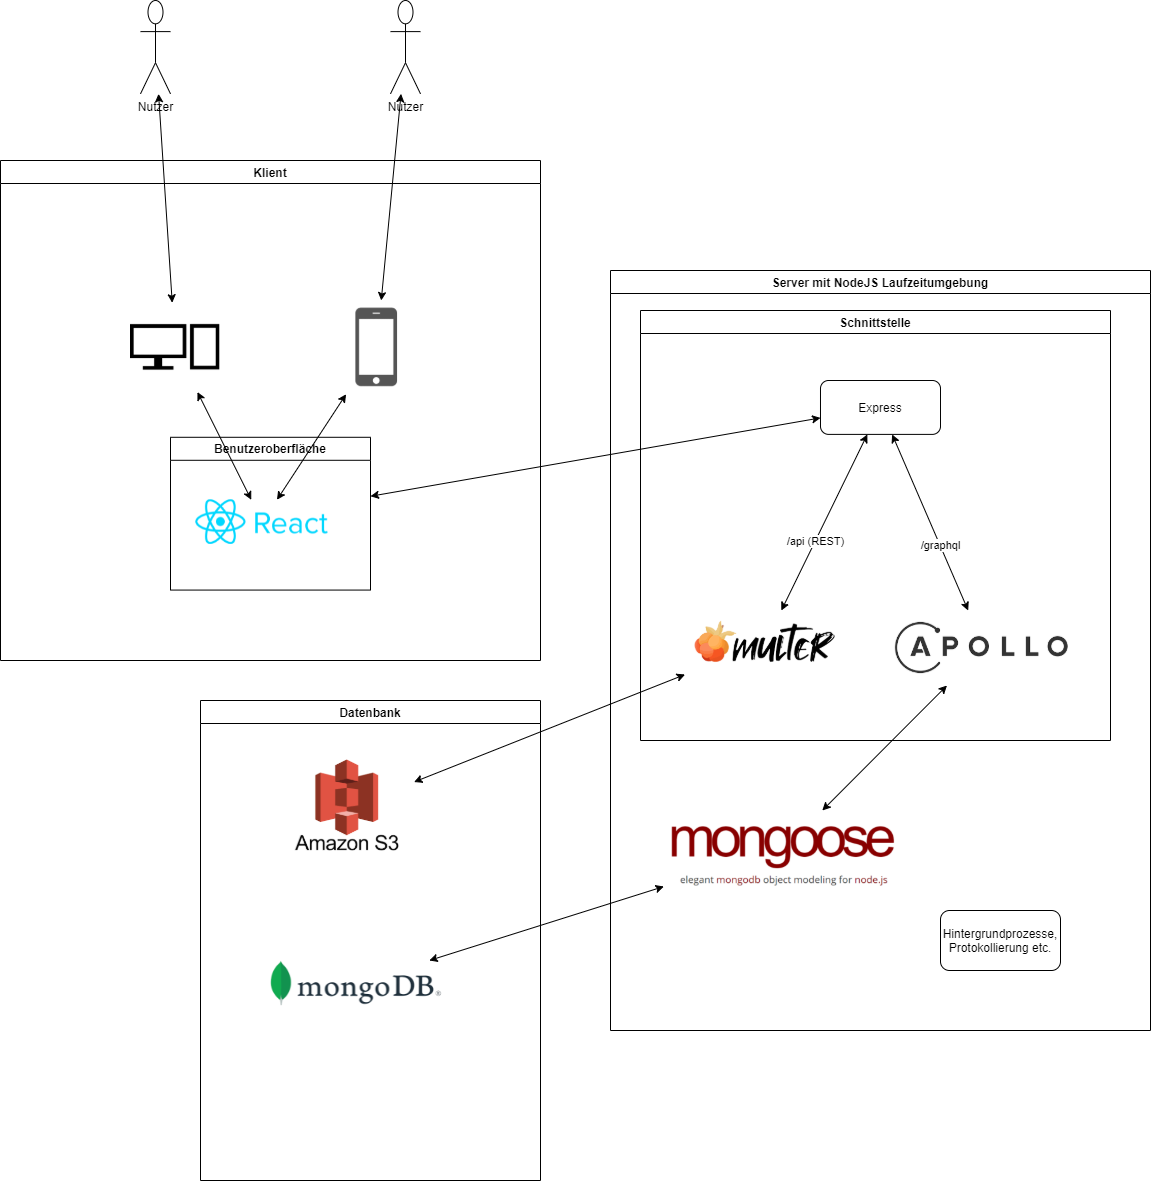
\includegraphics[width=\textwidth]{sources/MERN-Stack_Schaubild.drawio}
\begin{figure}[ht]
	\centering
	\caption{Die Interaktion der verwendeten Technologien als Schaubild}
	\label{figMERN1}
\end{figure}

\paragraph{}
Der Nutzer interagiert mit dessem Endgerät mit der durch React generierten Benutzeroberfläche.
Für dynamische Inhalte werden dazu Anfragen an das NodeJS-Backend gesendet.
Dieses verwaltet mithilfe von Express verschiedene Routen.
Bilder werden als Dateien über die Route \textit{/api} mit Multer auf AWS S3 gespeichert.
Sollten Daten der Datenbank benötigt werden, wird die Route \textit{/graphql} verwendet, bei denen über Apollo und Mongoose die entsprechende Abfrage an die MongoDB-Datenbank geschickt wird. 
Die Technologien sowie dessen Alternativen und die Gründe zur Entscheidung werden in den folgenden Kapiteln erläutert.


\newpage
\section{Datenbank}\label{kap_Datenbank}
\subsection{Anforderungen}
\paragraph{}
Es wird eine moderne Plattform entwickelt, auf der sich Nutzer ähnlich Social Media Profile anderer Nutzer anschauen und miteinander Chats führen.
Nutzer sollen in Echtzeit miteinander schreiben können und nahezu keine Wartezeit in Kauf nehmen müssen, um sich andere Profile anzeigen zu lassen.
Die Datenbank sollte eine geringe Ausfallwahrscheinlichkeit haben, da die Anwendung ohne Datenbankanbindung nur beschränkt nutzbar ist.
Bis auf statische Seiten wie die Homepage werden nahezu überall Datenbankabfragen benötigt.
Um eine potenziell große Anzahl an Nutzern in der Zukunft des Projektes verwalten zu können, sollte es Skalierungsmöglichkeiten geben.

\paragraph{}
Im Folgenden wird näher auf die Ziele der Datenbank eingegangen und die NoSQL Datenbank MongoDB mit PostgreSQL, welche repräsentativ für SQL basierte ORDBMS steht, verglichen. 

\subsubsection{Lese- und Schreibgeschwindigkeit}
\paragraph{}
Um eine möglichst gute Benutzererfahrung zu gewährleisten, wird versucht, die Wartezeit beim Laden der Webseite zu verringern.\\
Eine realistische Benutzeroberfläche aktualisiert sich erst, wenn die Datenbank antwortet und der Schreibzugriff genehmigt wurde.
Eine optimistische Benutzeroberfläche wiederum geht davon aus, dass der Schreibzugriff erfolgen wird und aktualisiert sich sofort.
Bem Benutzer wird bereits visuell der Erfolgsfall angezeigt, die Benutzererfahrung wird gesteigert.
Sollte der Schreibzugriff wider Erwarten fehlschlagen, wird der Status der Benutzeroberfläche zurückgesetzt und der Nutzer durch eine Fehlermeldung informiert.
Im Gegensatz zu einer realistischen Benutzeroberfläche, welche sich erst aktualisiert, wenn die Datenbank antwortet und der Schreibzugriff genehmigt wurde, erhält der Benutzer sofort eine Rückmeldung und muss nicht auf eine Antwort unseres Servers warten.\\
Anders als Schreibanfragen, welche mit einer Bestätigung oder Ablehung der Anfrage antworten, fordern Leseanfragen Daten an.
Wartezeiten bei Leseanfragen können daher nicht maskiert werden.\\
Um in einem späteren Entwicklungsschritt die Reduzierung der Wartezeiten durch eine optimistische Benutzeroberfläche zu ermöglichen, werden daher langsamere Schreibgeschwindigkeiten in Kauf genommen, wenn sich mit dieser Entscheidung die Lesegeschwindigkeit erhöht.

\paragraph{}
Es bietet sich an, SQL-Datenbanken wie PostgreSQL in eine Normalform zu bringen, um das Aktualisieren und Einfügen von Daten zu beschleunigen und die Konsistenz und Integrität gemäß ACID zu wahren.
Normalisierung kann sich jedoch auch negativ auf die Lesegeschwindigkeit auswirken.
Daten in einer Normalform befinden sich in verschiedenen Tabellen, die bei Abfragen oft zusammengeführt werden müssen.
Die Anfragen werden dadurch komplexer und die Effizienz von Indexen nimmt ab.
Um die Lesegeschwindigkeit zu erhöhen kann Denormalisierung verwendet werden, bei denen die Daten für verschiedene Tabellen dupliziert werden.
Dabei muss darauf geachtet werden, dass bei einer Aktualisierung der Datensätze alle Kopien aktualisiert werden, um Anomalien und Datenverlust zu vermeiden \cite{db:denormalization}.
Dies führt zu mehr Aufwand im Schreiben des Quellcodes und sorgt damit für Zeitaufwand.


\paragraph{}
MongoDB speichert Dokumente im JSON-Format und ermöglicht es, mehrere Werte für einen Schlüssel in Form eines Arrays zu hinterlegen.
Auch ist es möglich, Dokumente in andere Dokumente einzubetten. \cite{db:mongoEmbeddedDocuments}
Dies beschleunigt Leseabfragen, da die angeforderten Daten meist bereits in einem Dokument vorliegen.
Allerdings verringert sich die Schreibgeschwindigkeit, da Daten meist redundant in mehreren eingebetteten Dokumenten vorliegen und bei einer Änderung an mehreren Stellen überschrieben werden müssen.\\
Anders als PostgreSQL ist MongoDB auf Grundlage dieser Art der Denormalisierung entworfen und ändert bei einem Schreibzugriff automatisch alle Instanzen des gleichen Dokumentes als Teil einer atomaren (Alles-oder-Nichts-)Transaktion.
Auch Multi-Dokument-Transaktionen über verschiedene Shards und Replikatgruppen sind optional atomar. \cite{db:mongoAcidCompliance}

\subsubsection{Flexible Datenstrukturen}
Im Rahmen des \textit{(Minimum Viable Product) MVPs} stehen die Projektanforderungen fest, allerdings soll im späteren Verlauf des Projektes auf die Wünsche der Nutzer geachtet und entsprechende Anpassungen an der Anwendung getätigt werden.
Datenstrukturen werden verworfen und angepasst, wenn sich diese nicht als nützlich erweisen.
Speziell in der Anfangsphase eines Teilprojektes erlauben flexible Datenstrukturen eine Lösung zu entwickeln, welche mit wenig Zeitaufwand ein akzeptables Ergebnis liefert.
Sollte sich das Teilprojekt als erfolgreich erweisen, kann in einem späteren Entwicklungsschritt die Lösung inkrementell verbessert werden.
Eine Datenbank, die sich flexibel verändern lässt, ermöglicht es, schneller Anpassungen durchzuführen und verkürzt damit die Entwicklungszeit.

\paragraph{}
Tabellen in PostgreSQL können mit DDL-Befehlen wie ALTER TABLE verändert werden. \cite{db:postgresAlterTable}
Spalten können hinzugefügt, entfernt oder verändert werden, durch bestehende Constraints (\enquote{Zwangsbedingungen} / \enquote{Beschränkungen}) wird das Entfernen oder Ändern spezieller Spalten in einigen Fällen von der Datenbank verhindert, um die Integrität der Daten zu gewährleisten. 
Das Ändern des Datentyps einer Spalte ist in der Regel nur möglich, wenn die Datentypen zueinander kompatibel sind (z.B Wechsel eines Ganzzahl-Datentyps zu einem anderen, der mehr Speicherkapazität bietet) oder die Spalte für alle Datensätze leer ist.
Das Ändern von bestehenden Spalten kann, unter anderem durch Constraints, zu Problemen führen, die mit einem weiteren Zeitaufwand einher gehen.

\paragraph{}
MongoDB speichert Dokumente in Kollektionen, Dokumente der gleichen Kollektion müssen nicht die gleiche Struktur aufweisen. \cite{db:mongoCollection}
Dies ist möglich, da das Dokument dessen Struktur nach JSON-Spezifikation (durch die Angabe der Schlüssel-Wert-Paare) selbst beinhaltet.
Dem\-entsprechend können Dokumente mit neuen, anderen oder fehlenden Attributen direkt zu bestehenden Kollektionen hinzugefügt werden.
Dies erlaubt es, bei der Weiterentwicklung von Kollektionen direkt die neuen Dokumente in bestehende Kollektionen einzufügen, ohne bestehende Dokumente verändern zu müssen.
Es wird Zeit gespart und im Falle eines Fehlers lässt sich die Transaktion zurückrollen.
Es sollte Wert auf die Abwärtskompatibilität gelegt werden, damit bestehende Schnittstellen ohne Veränderung weiter funktionieren.

\subsubsection{Skalierbarkeit}
Mit jedem neuen Nutzer der Plattform steigt die Diversität und somit die Chance, dass sich zwei Nutzer finden, welche zusammenpassen und sich anfreunden.
 Je mehr Teilnehmer dem Netzwerk angehören, desto höher ist die Anzahl der potenziellen Kommunikationspartner und somit der Nutzen und Wert der Plattform.
Es handelt sich somit um einen positiven direkten Netzwerkeffekt. \cite{db:networkEffect}
Je größer der Nutzen der Anwendung, desto eher werden Benutzer weitere Nutzer anwerben, wodurch die Nutzerbasis wächst und der Nutzen steigt.
Dies kann zu exponentiellem Wachstum führen. \cite{db:networkEffectExponential}
Desweiteren können große Persönlichkeiten der sozialen Medien (\enquote{Influencer}) mit einer einzigen Bemerkung tausende Personen davon überzeugen, sich die Anwendung zu testen. \\
Eine kurzfristige, rapide Vergrößerung der Nutzerbasis und exponentielles Wachstum stellen Datenbanken vor eine Herausforderung, die sich mit Skalierung lösen lässt.
Auch sollen die Kapazitäten der Datenbank flexibel verringert werden können, um in Zeiten, in denen die Datenbank nicht ausgelastet ist, finanzielle Mittel zu sparen.
Zur Skalierung wird eine Kombination aus vertikaler Skalierung (leistungsfähigere Hardware) und horizontaler Skalierung (mehr Geräte nebeneinander betrieben) gewählt.
Vertikale Skalierung stößt auf Limitierungen, da der Preis von leistungsfähiger Hardware exponentiell skaliert. \cite{db:verticalScaling}
Weitere Skalierung ist dann nicht mehr rentabel. \\
Bei horizontaler Skalierung müssen die einzelnen Knoten miteinander kommunizieren.
Die für die Kommunikation benötigten Ressourcen steigen mit jedem weiteren Knoten.
Aus diesem Grund limitieren manche Datenbanken die Maximalanzahl an Knoten in einer Replikatgruppe. \cite{db:mongoReplicaSetElections}\\
Desweiteren kann Datenbanksharding, eine Art der Datenbankpartitionierung, betrieben werden, bei dem eine Datenbank in mehrere Splitter bzw. Scherben aufgeteilt wird, welche jeweils einen Teil der Daten verwalten.
Jeder dieser Splitter bildet wiederum eine eigene Replikatgruppe mit Primärknoten, Sekundärknoten und optional weiteren Knoten für Backups, Reportingtools und weitere. \cite{db:mongoHiddenReplicaSetMembers} \cite{db:mongoDelayedReplicaSetMembers} \cite{db:mongoReplicaSetArbiter}
Durch diese Verfahren können Datenmengen verarbeitet werden, welche die Kapazität einer einzelnen Replikatgruppe übertreffen würde. \cite{db:sharding}

\paragraph{Vertikale Skalierung\\}
Sowohl PostgreSQL als auch MongoDB lassen sich mit leistungsfähiger Hardware vertikal skalieren.
Zwischen den beiden Datenbanken gibt es dahingehend keine nennenswerten Unterschiede, die Datenbanken schneiden in diesem Punkt ähnlich ab.

\paragraph{Horizontale Skalierung\\}
Beide Datenbanken erlauben das Erstellen von Replikatgruppen mit einem Primärknoten, welcher für Lese- und Schreibzugriffe zur Verfügung steht und Sekundär- bzw. Standbyknoten, die je nach Einstellung entweder nur als Ausfallsicherheit dienen oder für Lesezugriffe zur Verfügung stehen.
MongoDB unterstützt horizontale Skalierung nativ, während für PostgreSQL weitere Pakete benötigt werden. \cite{db:mongoVsPostgres}
Das Aufsetzen von MongoDB gestaltet sich entsprechend einfacher.

\paragraph{Sharding\\}
\paragraph{}
Als SQL Datenbank werden bei PostgreSQL für komplexe DQL-Anweisungen \gls{DQL}, die Daten von mehreren Tabellen abfragen, JOIN-Answeisungen verwendet.
In einigen Fällen kann dies dazu führen, dass sich die abgefragen Spalten in verschiedenen Shards befinden.
Dies kann zu erhöhtem Aufwand bei Abfragen führen.
Um diesen Nachteil zu verringern, sollte darauf geachtet werden, wie die Shards konzipiert sind.
Durch eine kluge Aufteilung der Daten kann dafür gesorgt werden, dass bei einer Abfrage möglichst wenige verschiedene Shards abgefragt werden müssen.

\paragraph{}
MongoDB setzt auf Dokumente, welche in den meisten Fällen nicht auf Referenzen zu anderen Dokumenten angewiesen sind.
Dies wird unter anderem durch die Möglichkeit geschaffen, Dokumente in andere Dokumente einbetten zu können.
Infolgedessen entstehen weniger komplexe Abfragen, es müssen seltener Dokumente verschiedener Shards kombiniert werden.
Die Datenbank wird weniger beansprucht.
Auch erscheint das Erstellen von Shards mit MongoDB leichter als mit PostgreSQL.\\
Zusätzlich erlaubt Sharding bei international angelegten Projekten durch geschickte Wahl der Position der Datenbankknoten, die Latenzzeit bei Abfragen zu minimieren \autoref{fig:db:mongoActiveActive}.

\begin{figure}
	\centering
    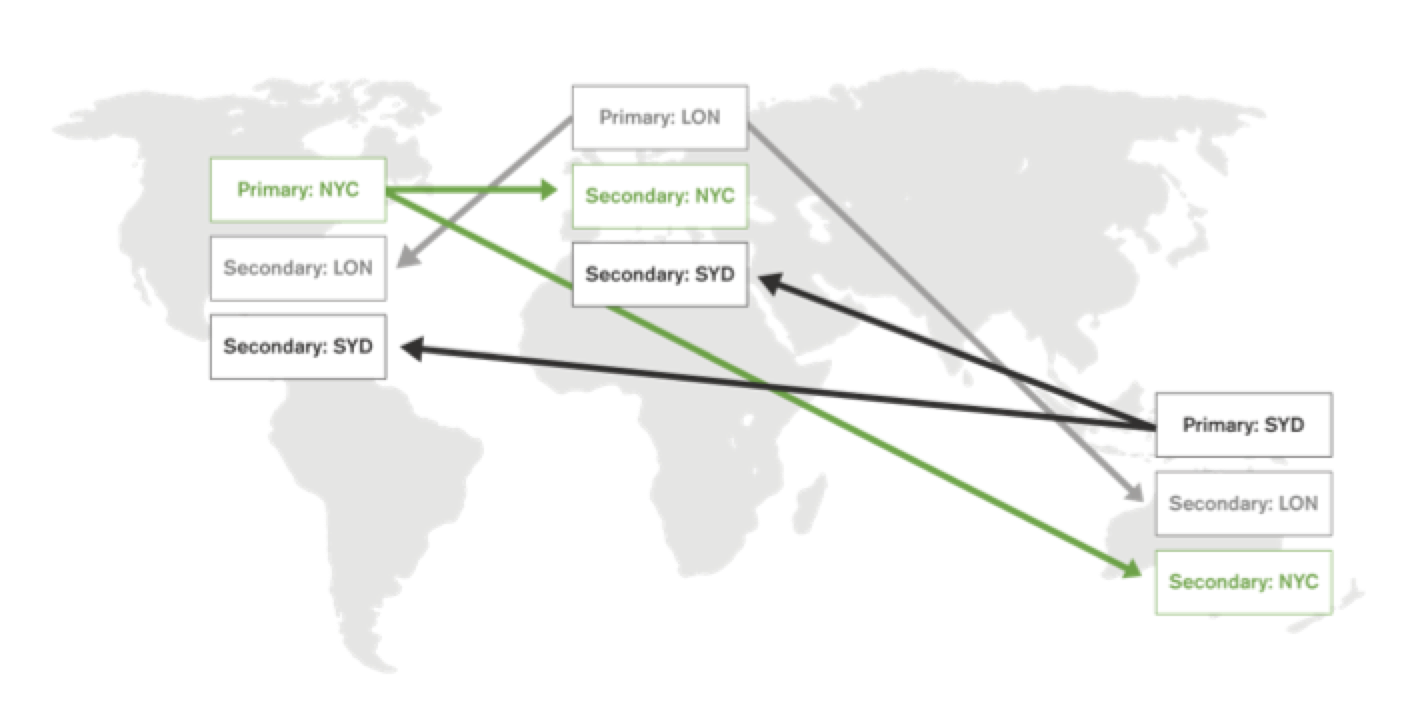
\includegraphics[width=\textwidth]{sources/MongoDB_sharded.png}\cite{db:mongoActiveActiveImage}
	\caption{Regionale Shards mit Replikatgruppen. Sekundärknoten befinden sich für niedrigere Latenzzeiten bei Lesezugriffen in anderen Regionen}
	\label{fig:db:mongoActiveActive}
\end{figure}

\subsubsection{Hochverfügbarkeit}
Für den Anmeldevorgang, die Registrierung und alle Seiten der Anwendung, die einen angemeldeten Nutzer voraussetzen, ist eine Datenbankanbindung zwingend erforderlich.
Sollten diese Dienste ausfallen, ist der Nutzen der Anwendung stark verringert.
Nur statische Seiten, wie die Startseite oder das Impressum, wären in so einem Fall verwendbar.
Dementsprechend bietet sich eine Datenbank mit Hochverfügbarkeit an, um das Risiko eines Ausfalls unserer Plattform so weit wie möglich zu verringern.\\
Um die Erreichbarkeit der Datenbank zu gewährleisten, bietet es sich an, Replikatgruppen zu erstellen.
Eine Replikatgruppe besteht aus mehreren Datenbankprozessen (Knoten), welche den gleichen Datensatz verwalten. \cite{db:mongoReplicaSetMembers}
Sollten durch Hardwarefehler einzelne Knoten ausfallen oder Softwarefehler Knoten dazu zwingen, neu gestartet zu werden, ist die Datenbank, wenn auch mit verringerter Leistung, weiterhin erreichbar.
Die dadurch erreichte Fehlertoleranz schafft Sicherheit und verringert drastisch die Chance, dass die Datenbank komplett ausfällt.\\
In der gewählten Konfiguration hat nur ein Prozess der Replikatgruppe Schreibrechte, um die Konsistenz bei gleichzeitigen Schreibzugriffen zu wahren.
Neben diesem Primärknoten existieren oft mehrere Sekundärknoten, welche die Schreibvorgänge des Primärknotens kopieren und für Lesezugriffe zur Verfügung stehen.\\
Es existieren andere Architekturen mit mehreren Primärknoten, die gleichzeitige Schreibzugriffe erlauben und besondere Herausforderungen bei der Datenkonsistenz stellen (\enquote{Multi-Master-Systeme}).
Diese werden hier nicht betrachtet.

\paragraph{}
PostgreSQL bietet verschiedene Lösungsansätze.
Bei synchronen Lösungen muss ein Schreibauftrag von allen Knoten durchgeführt sein, um als bestätigt zu gelten.
Asynchrone Lösungen erlauben einen Puffer zwischen dem Bestätigen eines Schreibauftrags und dessen Kopie auf andere Knoten.
Dadurch kann das Wechseln zu einem Backupknoten zu Datenverlust führen und Sekundärknoten können bei Lesezugriffen ein leicht veraltetes Ergebnis liefern.
Dafür gewinnt eine asynchrone Lösung an Performanz, da sich die Wartezeit verringert. \cite{db:postgresHighAvailability}\\
Um die Knoten auf dem gleichen Stand zu halten und im Fall eines Ausfalls Daten wiederherstellen zu können, wird ein \textit{Write-Ahead-Log} (WAL) angelegt, welcher unmittelbar nach jedem Commit die Transaktion in einen Transaktionslog schreibt.
Dieser wird dann von anderen Knoten ausgelesen und die Transaktion wird kopiert. \cite{db:postgresWriteAheadLogging}\\
Sollte der Primärknoten ausfallen, muss dies detektiert werden und ein Sekundärknoten mit so wenig Verzögerung wie möglich als neuer Primärknoten ausgewählt werden.
PostgreSQL bietet keine automatische Ausfallsicherung.
Es muss daher eine Drittanbietersoftware verwendet oder ein eigenes Skript geschrieben werden.
Um die Belastung der einzelnen Knoten möglichst gleich zu halten, sollte ein Prozess zur Lastverteilung existieren.
Für die Lastverteilung stehen einige Lösungen von Drittanbietern zur Verfügung.
Nach weitreichender Recherche konnte nicht ermittelt werden, ob PostgreSQL native Lastverteilung anbietet.
Allerdings gibt es verschiedene Projekte, welche Lösungen zur Lastverteilung anbieten. \cite{db:postgresLoadBalancing}


\paragraph{}
Knoten in MongoDBs Replikatgruppen teilen sich gegenseitig durch Ping-Befehle ihren \enquote{Herzschlag} mit, um zu ermitteln, ob ein Knoten ausgefallen ist.
Sollte der Primärknoten \enquote{sterben}, wählen die \enquote{überlebenden} Knoten in einer Abstimmung den nächsten Primärknoten, welcher die Schreibaufträge des vorigen Primärknotens übernimmt.
Der Prozess einer Wahl sollte in der Regel durchschnittlich nicht länger als 12 Sekunden dauern und passiert vollautomatisch \cite{db:mongoElectionTimeout}.
Einem Knoten mit mehr Leistung kann eine höhere Priorität zugewiesen werden, um diesen als präferierten Primärknoten zu definieren \cite{db:mongoElectionPriority}.
Auch eignet es sich, Knoten in anderen Regionen für die Rolle des Primärknoten als unwählbar zu definieren, da sich die Latenz ansonsten drastisch erhöhen würde.
Ein Replikset kann aus maximimal 50 Knoten bestehen, wovon bis zu 7 zum Primärknoten wählbar sind \cite{db:mongoReplicaSetMembersLimit}.
Diese Zahl ist vermutlich groß genug, um einen gleichzeitigen Ausfall aller Knoten aus technischer Sicht nahezu unmöglich zu gestalten, wenn sich die Knoten zusätzlich auf verschiedenen physischen Geräten befinden.\\
In seltenen Fällen kann es vorkommen, dass der Primärknoten ausfällt und vor seinem Ausfall Schreibaufträge bestätigt, diese aber nicht an die Standbyknoten weiterleiten kann. Wenn der frühere Primärknoten der Replikatgruppe wieder beitritt, in diesem Fall als Sekundärknoten, unterscheidet sich dessen Schreibhistorie von der anderer Knoten. Die Historie des früheren Primärknoten wird zurückgerollt und die bestätigten Schreibaufträge sind verloren. 
MongoDB versucht durch verschiedene Techniken, Rollbacks zu vermeiden und erlaubt es unter Verlust von Effizienz, mit Schreibbestätigungen erst zu antworten, wenn der Großteil der Replikatgruppe diese bestätigt hat. \cite{db:mongoRollback}\\
Leseanfragen werden per Standardkonfiguration an den Primärknoten gestellt, um möglichst aktuelle Daten liefern zu können.
Diese Präferenz lässt sich ändern, um den Primärknoten zu entlasten, auf speziell eingerichtete Knoten mit optimisierten Indexen zugreifen zu können, die Latenz zu verringern oder beim Ausfall des Primärknotens weiterhin Lesezugriffe zu ermöglichen. \\
Auch ist eine Wahl zwischen asynchronen und synchronen Operationen möglich.
Dabei sind asynchrone Operationen aufgrund der höheren Performanz die Standardeinstellung.

\paragraph{}
Aus den in diesem Unterkapitel genannten Gründen überzeugt MongoDB im Punkt der Hochverfügbarkeit gegenüber PostgreSQL.
Um PostgreSQL hochverfügbar zu machen, sind einige Anpassungen und Expertenwissen oder Drittanbietersoftware nötig.
MongoDB scheint von der Architektur auf Hochverfügbarkeit ausgerichtet zu sein und liefert Funktionen für eine automatische Ausfallsicherung, welche das System nach kurzer Zeit ohne manuelle Eingriffe wieder voll funktionstüchtig machen.
Es wird vermutet, dass mit MongoDB eine Datenbank eingerichtet werden kann, die mit wenig Aufwand stabil für sehr geringe Ausfallraten sorgen kann.

\subsubsection{Dateiformat}
MongoDB speichert Daten im JSON-Format. 
\enquote{JSON (JavaScript Object Notation) ist ein schlankes Datenaustauschformat, welches für Menschen einfach zu lesen und für Maschinen einfach zu parsen [\dots] ist} \cite{db:json}. 
JSON als semistrukturiertes Dateiformat eignet sich daher gut für Schnittstellendaten.\\
Desweiteren wird im gewählten MERN-Techstack ausschließlich JavaScript verwendet - das JavaScript native Dateiformat JSON ist daher ohne Umwandlungen direkt verwendbar und der Umgang für das Entwicklerteam bereits bekannt.
Dies verringert die Gefahr möglicher Komplikationen und spart Lern- und Programmieraufwand.
Diesen Vorteil besitzt PostgreSQL nicht.
Abfrageergebnisse müssen für die Schnittstelle zuerst in JSON-Dateien geändert werden, was einen zusätzlichen Programmierschritt bedeutet.

\subsubsection{Fazit}
\begin{table}
\centering
\begin{tabularx}{\linewidth}{ |X|X|X| } 
    \hline
    Kriterien & PostgreSQL & MongoDB  \\ 
    \hline
    Lesegeschwindigkeit & Mittel & Hoch \\
    Schreibgeschwindigkeit & Mittel & Langsam - Mittel \\
    Datenstrukturen & Strenges Tabellenschema & Schemafrei durch selbstbeschreibende JSON-Dokumente \\
    Skalierbarkeit & Meist vertikal, horizontal benötigt erweitertes Setup & Meist horizontal, unterstützt nativ Sharding \\
    Hochverfügbarkeit & Replikatgruppen, Lastverteilung und automatische Ausfallsicherung meist über Drittsoftware & native Replikatgruppen und automatische Ausfallsicherung, Lastverteilung bei Wahl eines Sekundärknotens, automatische Wahl des nächsten Primärknotens bei Ausfall \\
    Dateiformat & internes Format, wird bei Abfragen in lesbaren Tabellen ausgegeben & JSON \\
    \hline
\end{tabularx}
\caption{Vergleich PostgreSQL und MongoDB}
\label{db:table:comparisonPostgresMongo}
\end{table}

Es konnte gezeigt werden, dass beide Datenbanken eine ausgereifte Architektur besitzen und sich daher beide gut für Softwareprojekte eignen.
Für dieses Projekt bietet MongoDB einige Vorteile, die sich auf die Entstehungsgeschichte von MongoDB zurückführen lassen.\\
Die 2007 neu gegründete Firma 10Gen, mittlerweile bekannt als MongoDB Inc., benötigte eine Datenbank, welche den Anforderungen ihrer quelloffenen Plattform-as-a-Service Cloud-Architektur gerecht werden würde.
Das Team suchte nach einer Datenbank, die elastisch, skalierbar, einfach zu verwalten und für Entwickler und Anwender einfach zu benutzen ist.
Unzufrieden mit den zu der Zeit auf dem Markt verfügbaren Datenbanksystemen wurde MongoDB, eine dokumentbasierte Datenbank, entwickelt.
Als das Team das Potenzial der Datenbank realisierte, wurde die Idee der Cloud-Plattform eingestellt und die Entwicklung von MongoDB gefördert.\cite{db:mongoHistory}\\
Native Funktionen wie MongoDBs automatische Ausfallsicherung, horizontale Skalierung und Sharding lassen sich wenig Aufwand konfigurieren und skalieren.
Bei der Anwendung werden auf einen komplexen Schreibzugriff vermutlich dutzende bis hunderte Lesezugriffe kommen.
Dementsprechend sorgt die schnellere Lesegeschwindigkeit zu Kosten der Schreibgeschwindigkeit für schnellere Datenbankzugriffe.
Zudem integriert sich das von MongoDB gewählte Dateiformat JSON gut mit der weiteren Architektur des verwendeten MERN-Techstacks.
Aus den genannten Gründen fällt die Wahl der Datenbank für das Projekt auf MongoDB.


\subsection{Schemata}
MongoDB organisiert Daten in Kollektionen.	
Folgende Kollektionen wurden verwendet, um die Daten optimal zu verwalten:

\paragraph{Nutzer}
\begin{table}
    \centering
    \begin{tabularx}{\textwidth}{ |X|X|X| } 
        \hline
        Feld & Beschreibung & Beispiel \\ 
        \hline
        Id & Standardmäßige MongoId & \\
        Benutzername & einzigartiger, öffentlicher Name & MaxMustermann \\ 
        normalisierter Name & Name in Kleinbuchstaben. Wird verwendet, um die Einzigartigkeit von Namen zu gewährleisten & maxmustermann \\ 
        Email & private eMail des Nutzers & mustermann@email.de \\
        Rolle & Gibt an, ob der Nutzer autorisiert ist - Moderatoren und Administratorkonten haben mehr Rechte. Automatisch generiert & Nutzer \\ 
        Geburtsdatum & privates Geburtsdatum des Nutzers & 01.01.2000 \\ 
        Alter & Alter des Nutzers. Wird automatisch mit Geburtsdatum berechnet & 21 \\ 
        Sprachen & Array von Sprachen, die der Nutzer sprechen kann & {[de, en]} \\
        Geschlecht & gesellschaftliches Geschlecht des Nutzers. & Männlich \\ 
        Spielposition & Bis zu 2 Lieblingspositionen des Spielers in League of Legends & {[Mid, Jungle]} \\ 
        Freitext & kurzer Text, in dem der Nutzer sich beschreiben kann. & Ich bin ein toller Nutzer! \\
        Avatar & URI vom Avatarbild des Nutzers & \url{https://<s3-name>.s3.eu-central-1.amazonaws.com/avatars/<UUID>.jpg} \\ 
        Freunde & Array von allen Freunden des Nutzers. Beinhaltet die NutzerID und die ChatID & {[[id1, NutzerID1, ChatID1], [id2, NutzerID2, ChatID2]]}\\ 
        Geblockt & Array von NutzerIDs der Nutzer, die geblockt wurden & {[NutzerID3, NutzerID4]} \\ 
        \hline
    \end{tabularx}
    \caption{Schema Nutzer}
    \label{db:table:nutzer}
\end{table}

Wenn ein Nutzer einen Account erstellt, gibt dieser seine Email-Adresse, den gewünschten Benutzernamen und das gewünschte Passwort an. 
Durch Indexe wird die Einzigartigkeit von eMail und Benutzername geprüft, das Passwort wird aus Sicherheitsgründen in einer separaten Kollektion gespeichert.
Nach der Kontoerstellung kann der Nutzer das Geburtsdatum, die gesprochenen Sprachen, das Geschlecht, die Spielposition und einen Freitext angeben sowie ein Bild hochladen, welches als Avatarbild dient.
Felder wie der normalisierte Name, das Alter und die Rolle werden automatisch generiert.
Im Laufe der Nutzung der Plattform wird der Nutzer andere Spieler als Freunde hinzufügen - diese werden in einer Freundesliste gespeichert.
Auch steht es dem Nutzer frei, Andere zu blockieren - in diesem Fall wird die NutzerID des Blockierten auf die Blockliste hinzugefügt. \\
Privatsphäre und damit die Sicherheit der eigenen Daten stellt einen hohen Stellenwert dar.
Die Anzahl an Daten, die ein Nutzer von sich preisgeben muss, soll so gering wie möglich halten werden.
Die Email-Adresse, das Geburtsdatum und Freundes- und Blockliste sind für andere Nutzer nicht einsehbar.
Bis auf den Benutzernamen, bei welchem es sich um einen Fantasienamen handeln kann, muss eine Person keine Daten öffentlich angeben.

\paragraph{Sprache\\}
Damit Nutzer ihre gesprochenen Sprachen wählen können, bieten wir die Wahl zwischen 187 Sprachen nach ISO 639-1 Norm an.\cite{db:iso639-1}\\

\begin{table}
    \centering
    \begin{tabular}{ |c|c|c| }
    \hline
        Feld & Beschreibung & Beispiel \\
        \hline
        Id & Alpha-2 Code der Sprache & en, de, fr \\
        Name & Englische Schreibweise der Sprache & English, German, French \\
        nativer Name & native Schreibweise der Sprache & English, Deutsch, français \\
        \hline
    \end{tabular}
    \caption{Schema Sprache}
    \label{db:table:sprache}
\end{table}

Standardmäßige Objekt-IDs von MongoDB enthalten einen Zeitstempel und einen inkrementellen Zähler \cite{db:mongoObjectId}.
 Diese Daten sind bei Sprachen - öffentlichen Stammdaten, die sich über einen langen Zeitraum nicht verändern werden - nicht relevant.
Stattdessen wurde der Alpha-2-Code der Sprache als ID gewählt, der in den meisten Fällen auf die Sprache schließen lässt.
Nutzerdokumente referenzieren die Sprache per ID.
Dadurch fällt es leichter, direkt im Nutzerdokument anhand der Sprach-ID zu erkennen, welche Sprachen der Nutzer spricht.
Auch wird das manuelle Kontrollieren von Testfällen hierdurch vereinfacht.
Sprachen können sowohl anhand der englischen Schreibweise als auch der nativen Schreibweise gefunden werden.
Dies erleichtert auch nicht-englischsprachigen Nutzern, ihre Sprache auswählen zu können.

\paragraph{Passwort\\}
\begin{table}
    \centering
    \begin{tabular}{ |c|c| }
        \hline
        Feld & Beschreibung  \\
        \hline
        Id & Standardmäßige MongoId \\
        Passwort & Bcrypt Hash des Passworts bestehend aus Versionsnummer, Komplexität, Salt und Hash \\
        NutzerID & MongoId des zugehörigen Nutzers \\
        \hline
    \end{tabular}
    \caption{Schema Passwort}
    \label{db:table:passwort}
\end{table}

Das Passwort wird nicht im Nutzerdokument gespeichert, da sonst schon kleine Programmierfehler dazu führen könnten, dass normale Nutzer das gehashte Passwort anderer Nutzer ermitteln könnten.
Um dieses Sicherheitsproblem direkt zu eliminieren, wird daher für jedes Passwort ein eigenes, vom Nutzerdokument isoliertes Dokument verwendet.\\
Das Passwort wird durch bcrypt, einem Blowfish-basierten Einweg-Hashalgorithmus, auf der Datenbank als Hash mit Salt gespeichert.
Die Komplexität des Hashes ist frei wählbar und neben Versionsnummer, Salt und dem Hash an sich in der Zeichenkette gespeichtert.\cite{db:bcrypt}\\
Bei der Wahl der Komplexität ist die Sicherheit gegen Rechengeschwindigkeit abzuwägen.
Eine höhere Komplexität erhöht die benötigte Zeit pro Versuch eines Angreifers, das Passwort zu knacken.
Gleichzeitig wird aber auch die Zeit, die unser Server benötigt, um ein neues Passwort zu generieren oder den Anmeldeversuch eines ehrlichen Nutzers zu bestätigen, erhöht.
Eine zu hohe Komplexität kann daher den Server stark verlangsamen und macht Angriffszenarien per (D)DOS ((distributed) denial of service, Überlastung des Servers durch übermäßigen Datenverkehr) gefährlicher, da gezielte Anmeldeversuche viel Last auf dem Server erzeugen.
In Zukunft werden weitere Limitierungen auf Seiten des Backends erstellt, um wiederholte Anmeldeversuche zu bremsen.\\

Zur Verringerung des Erfolges von Brute-Force-Angriffen wird verlangt, dass das Passwort aus mindestens 8 Zeichen, darunter mindestens jeweils 1 Großbuchstabe, 1 Kleinbuchstabe und 1 Ziffer, erstellt wird.
Für mehr Varianz in den Passwörtern sind zudem einige Sonderzeichen erlaubt.
Es besteht eine 1:1-Relation zwischen Passwörtern und Nutzerkonten.

\paragraph{Verhältnis\\}
\begin{table}
    \centering
    \begin{tabular}{ |c|c| }
        \hline
        Feld & Beschreibung  \\
        \hline
        Id & Standardmäßige MongoId \\
        Sender & NutzerID der Person, die den Like/Dislike versendet. \\
        Empfänger &  NutzerID der Person, die den Like/Dislike empfängt. \\
        Status & Gibt an, ob es sich um einen Like oder Dislike handelt. \\
        \hline
    \end{tabular}
    \caption{Schema Verhältnis}
    \label{db:table:like}
\end{table}

Immer wenn ein Nutzer bei der Kontaktsuche angibt, ob er mit einer Person Kontakt aufnehmen oder diesen vermeiden will, wird ein Dokument angelegt. 
Wenn der Nutzer in Kontakt treten möchte, wird zusätzlich geprüft, ob bereits ein Datensatz existiert, bei dem Sender und Empfänger vertauscht sind - ob sich also die Nutzer gegenseitig einen Like gegeben haben. 
In diesem Fall werden beide Datensätze gelöscht und die Nutzer zur Freundesliste des jeweils anderen hinzugefügt und ein Dokument der Kollektion Chat erstellt. 
Die Nutzer können ab dann miteinander kommunizieren. 
Dislikes sorgen dafür, dass ein Kontakt in Zukunft nicht mehr möglich ist.

\paragraph{Chat\\}
\begin{table}
    \centering
    \begin{tabular}{ |c|c| }
        \hline
        Feld & Beschreibung  \\
        \hline
        Id & Standardmäßige MongoId \\
        Teilnehmer & Array von NutzerIDs, die dem Chat beiwohnen. Aktuell maximal 2. \\
        Nachrichten & Array von Nachrichten, die die Nutzer untereinander ausgetauscht haben. \\
        \hline
    \end{tabular}    
    \caption{Schema Chat}
    \label{db:table:chat}
\end{table}

Sollten sich zwei Nutzer befreunden, wird zwischen diesen ein Chat erstellt.
Wenn ein Nutzer die Freundschaft beendet, verlässt dieser gleichzeitig den Chat. 
Mit der gewählten Struktur sind auch Gruppenchats ohne Änderung der Datenbank möglich, falls dies in Zukunft eine erwünschte Funktionalität sein sollte.\\
Um Ressourcen zu sparen, wird bei der Standard-Datenbankabfrage nur die neueste Nachricht geladen.
Diese Abfrage dient für Vorschaubilder des Chats in der Kontaktliste.
Außerdem ist es möglich, durch Pagination (Seitennummerierung) je Abfrage 20 Nachrichten zu erfragen.
Diese Methoden verringern die Serverlast, da in vielen Fällen nicht mehr als die erste Seite der Abfrage relevant ist.\\

\subparagraph{Nachricht\\}
Nachrichten sind eingebettete Dokumente eines Chats.
Sie weisen folgende Datenstruktur auf:

\begin{table}
    \centering
    \begin{tabular}{ |c|c| }
        \hline
        Feld & Beschreibung  \\
        \hline
        Id & Standardmäßige MongoId \\
        Inhalt & Text der Nachricht \\
        Autor & NutzerID des Verfassers der Nachricht \\
        \hline
    \end{tabular}
    \caption{Eingebettetes Schema Nachricht}
    \label{db:table:nachricht}
\end{table}

\subsection{Database-as-a-Service}
Um eine Datenbank selbst zu betreiben fehlt es dem Projekt an fachlichen Kapazitäten und einer Infrastruktur, welche physische Datenbankserver unterstützt.
Es bietet sich daher eine Database-as-a-Service-Lösung (DBaaS) an.\\ 
MongoDB Inc. bietet mit MongoDB Atlas eine DBaaS an, die flexibel auf die Größe und Auslastung des Projektes angepasst werden kann.
Dazu gibt es verschiedene Datenbankstufen, die mit höheren Kosten mehr Rechenleistung und weitere Funktionen erhält.
Zwischen den Stufen kann flexibel gewechselt werden, um den realen Auslastungen gerecht zu werden.
Kostenpflichtige Stufen bieten die Möglichkeit an, Backups einzurichten.
Für höhere Kosten stehen außerdem Werkzeuge zur Verfügung, die Metriken in Echtzeit anzeigen, automatisch archivieren, Empfehlungen zur Leistungsoptimierung erstellen oder langsame Datenbankabfragen zur Diagnose und Optimierung anzeigen.
In der Entwicklungsphase wurde sich für die kostenlose Stufe entschieden, da die Funktionen und Leistung für die Entwicklungsumgebung ausreichen.
Sollte das Produkt auf den Markt gehen, wird auf eine kostengünstigste Stufe gewechselt, um die Option von Backups zu erhalten.
Sollte das Projekt erfolgreich sein und viele Nutzer anziehen, wird flexibel, abhängig von der benötigten Leistung, eine teurere Stufe mit mehr Leistung gewählt.\\
Sowohl die Produktions-, als auch die Entwicklungsumgebung werden als eigene Datenbanken von MongoDB Atlas gehosted (host = Gastgeber, Betrieb der Datenbank durch MongoDB Atlas, Zugriff auf diese über das Internet).
Dies verringert das Risiko von Code, der auf der lokalen Maschine funktioniert, aber auf der Produktionsumgebung Fehler wirft.
Durch die Nutzung gleicher Werkzeuge und gleicher Technologie wird die Werkzeuglücke verringert und dementsprechend die Dev-Prod-Vergleichbarkeit erhöht. \cite{db:devProdParity}

\subsection{Avatarbilder}
Statt Bilddateien für Avatare direkt auf der Datenbank zu speichern, was mit langen Wartezeiten auf die Datenbank einhergehen würde, werden nur die URIs zu den Bildern auf der Datenbank gespeichert.
Für das Speichern der Binärdateien wurde sich für AWS S3 entschieden, einem Speichersystem, welches für BLOB-Dateien (Binary Large OBject) optimiert ist.
Dies nimmt der Datenbank Last ab und erhöht die Anfragegeschwindigkeit bei Lese- und Schreibzugriffen des Avatarbildes.\\
Der S3-Speicher wurde so eingerichtet, dass das Backend Zugriffsrechte zum Erstellen und Löschen von Dateien hat.
Beim Verteilen der Zugriffsrechte wurde nach Minimalprinzip vorgegangen.
Das Backend besitzt nur die minimal nötigen Zugriffsrechte und keine weiteren.
Ein möglicher Angriff verursacht dadurch weniger Schaden, als wenn das Backend alle Zugriffsrechte hätte.\\
Die Datenbank wird mithilfe von GraphQL angesprochen, für S3 hat sich diese Lösung jedoch nicht angeboten.
Für das Hochladen von Profilbildern wurde eine weitere Route im Backend erstellt, bei der mit den npm-Paketen Multer und Multer-S3 kontrolliert wird, ob es sich bei der vom Nutzer hochgeladenen Datei um eine Bilddatei handelt und ob diese eine bestimmte Bildgröße nicht übersteigt.

\subsection*{Fazit}
Mit den gewählten Kollektionen und der Wahl von speziellen Hosts sind wir in der Lage, Nutzern eine Datenbank anzubieten, die eine hohe Erreichbarkeit aufweist, sich leicht an die Auslastung skalieren lässt, personenbezogene Daten geheim hält und ein Maß an Datensicherheit bietet, welches der Größe des Projektes entspricht.
Flexible Datenstrukturen erlauben schnelle Anpassungen des Projektes.
Die Verwendung eines bekannten Dateiformats, welches sich gut für Schnittstellen eignet, sorgt für Zeitersparnisse in der Entwicklung des Frontends und der Datenbankschnittstelle und reduziert somit den Aufwand.
Außerdem werden durch eingebettete Dokumente, Denormalisierung und Seitennummerierung Optimierungen durchgeführt, die als Ziel haben, möglichst schnell Antworten auf Leseanfragen zu bieten.

\newpage
\section{Backend}\label{kap_Backend}
Das Backend stellt Endpunkte bereit, die in der Lage sind, auf HTTP-Anfragen zu antworten.
Damit dient das Backend unter anderem als Bindeglied zwischen Frontend und Datenbank.
Auch können durch verschiedene Funktionen Nutzer autentifiziert und autorisiert werden.
Dies ist für manche Datenbankabfragen, wie zum Beispiel das Ändern des eigenen Profils, Voraussetzung.

\subsection{Node}
\paragraph{}
NodeJS ist eine JavaScript Laufzeitumgebung, die es ermöglicht, JavaScript Code auf einem Server auszuführen \cite{be:node}.
Der Server beantwortet die Abfragen, welche vom Nutzer über das Frontend verschickt werden und verwaltet die Routen der Domäne, um den gewünschten Inhalt anzeigen zu können.
Mit der Hilfe von Paketverwaltungswerkzeugen wie npm ist es möglich, Programmierpakete in das Projekt einzubinden \cite{be:npm}.\\

\paragraph{}
Der Kommandozeilenbefehl \textit{node start} wird ausgeführt, um das Hauptprogramm \textit{server.js} auszuführen.
Das verwendete \textit{dotenv}-Paket erlaubt es, eine Datei mit dem Namen \textit{.env} zu erstellen, mit der Umgebungsvariablen definiert werden \cite{be:dotenv}.
Die Datei wird nicht durch git verfolgt, da sonst geheime Informationen wie Passwörter und Zugriffsschlüssel öffentlich wären.
Diese komprommitierten Daten würden Angreifern leichten Zugriff in das System geben.
Durch die Verwendung des Paketes können zudem verschiedene Umgebungsvariablen für Entwicklungs-, Test- und Produktionsumgebung verwendet werden.\cite{be:dotenv2}\\

\paragraph{}
Nach der Definition der Umgebungsvariablen verbindet sich der Node-Server mit der Mongo-Datenbank.
Dazu wird im verwendeten Paket \text{Mongoose} eine URL angegeben, welche einen Anmeldeschlüssel enthält \cite{be:mongoose}.
Zuletzt werden die Express- und Apollo-App gestartet und der Server danach endgültig aktiviert.

\subsection{Express}
Das minimalistische
Paket ExpressJS erlaubt die Definition von Routen und Middleware \cite{be:express}\cite{be:expressRouting}\cite{be:expressMiddleware}. \\

\subsubsection{Routen}
Routen geben an, welcher Inhalt bei einer HTTP-Anfrage zurückgegeben werden soll.
Die Express-Funtkionen definieren, auf welche REST-Methode (GET,POST,\dots) und auf welchem Pfad diese ausgeführt werden sollen.
Die Funktion hat Zugriff auf die Anfrage des Nutzers (request) und erstellt daraufhin eine Antwort (response).


\paragraph{Root ('/')\\}
Bei einer GET-Anfrage auf das Stammverzeichnis wird mit \enquote{Hello World!} geantwortet.
\begin{lstlisting}
    app.get('/', (request, response) => {
        response.send('Hello World!')
    })
\end{lstlisting}
In Zukunft wird hier mit der Homepage geantwortet werden, auf der das Projekt beschrieben wird.
Aktuell dient die Route als Platzhalter.

\paragraph{/graphql\\}
Eine Anfrage an die Route \textit{/graphql} wird von Apollo, dem gewählten Framework für GraphQL, beantwortet.
Der Großteil aller Abfragen an das Backend gehen an diesen Endpunkt.
Durch die für Apollo getätigten Einstellungen ist GraphiQL aktiviert, eine graphische Oberfläche, die die Benutzung der Datenbankschnittstelle erleichtert.
Durch Introspektion (eine Apollo-Einstellung) steht eine umfangreiche Dokumentation der möglichen Abfragen und deren Datentypen zur Verfügung.
Dies erleichtert das Schreiben von Schnittstellenabfragen.
Genauere Informationen zu GraphQL und Apollo sind in dem entsprechenden Kapitel zu finden.

\paragraph{/api\\}
GraphQL unterstützt nativ nur eingeschränkte Möglichkeiten zum Hochladen von Multipart-Dateien wie Bildern \cite{be:graphQlTypes}.
Es wurde sich daher für einen klassischen REST-Endpunkt entschieden.
Mit Hilfe des Paketes Multer werden die Bilddateien auf AWS S3 gespeichert \cite{be:multer}\cite{be:multerS3}.
Die Autorisierung von AWS wird dabei durch das Paket \textit{aws-sdk} gelöst.\\

Zum Erstellen von Profilbildern wird die Subroute \textit{/avatar} verwendet.
Mit Hilfe von Multer werden verschiedene Regeln definiert, welche prüfen, ob es sich bei der hochgeladenen Datei um ein Bild handelt und die maximale Dateigröße nicht überschritten wird.
Sollten alle Prüfungen erfolgreich sein, wird das Bild mit einem durch UUID Version 4 generiertem Dateinamen auf S3 hochgeladen.
Damit das Bild öffentlich verfügbar ist, muss die Zugriffskontrollliste von AWS für das Bild auf \enquote{öffentlich lesbar} gesetzt werden.
Zum Schluss wird die URL des generierten Bildes im Nutzerdokument abgelegt, um eine Referenz auf das Bild zu erhalten.\\

Die Route \textit{/avatar} steht nur für POST-Anfragen zur Verfügung.
Für die Äquivalente GET-Abfrage wird die GraphQL-Schnittstelle verwendet.
Dies ist möglich, da nur die URL der AWS-Datei, aber nicht das Bild selbst zurückgegeben wird.
Die URL wird dann im HTML-Dokument vom Nutzer geöffnet.\\

In Zukunft können weitere Subrouten für \textit{/api} erstellt werden, die zum Beispiel mit \textit{Multer} in der Lage sind, auf Schnittstellenabfragen zu antworten.
Eine mögliche Funktionalität wäre das Hochladen von Bildern in Chats.
Hier würden AWS S3 und Multer wieder zur Verwendung kommen, da die Anforderungen denen von \textit{/avatar} größtenteils entsprechen.

\subsubsection{Middleware}
\enquote{Middlewarefunktionen sind Funktionen, die Zugriff auf das Anforderungsobjekt (req), das Antwortobjekt (res) und die nächste Middlewarefunktion im Anforderung/Antwort-Zyklus der Anwendung haben. Die nächste Middlewarefunktion wird im Allgemeinen durch die Variable next bezeichnet.}\cite{be:expressMiddlewareQuote}
Middlewarefunktionen lassen sich sowohl auf Anwendungsebene als auch für einzelne Routen definieren.
Mögliche Ziele der Funktionen sind: Die Protokollierung von Webseitenzugriffen, die Autorisierung von Anfragen und die Blockierung von fehlerhafte Anfragen.

\paragraph{CORS\\}
Per Same-Origin-Poicy (SOP) sind Zugriffe von einer Domäne auf die andere normalerweise nicht gestattet \cite{be:mdnSop}.
Dies unterbindet Abfragen des Frontends an das Backend, da Frontend und Backend unter verschiedenen Servern laufen.
Durch CORS (Cross-Origin Recource Sharing) können Ausnahmen für SOP erstellt werden \cite{be:mdnCors}.
Eine vom Express-Paket gelieferte Middleware wird verwendet, welche es erlaubt, CORS zu aktivieren \cite{be:expressMiddlewareCors}.

\paragraph{JWT\\}
Einige Daten der Datenbankschnittstelle sind öffentlich verfügbar.
Manche Daten, wie zum Beispiel private Nutzerdaten, benötigen stattdessen eine Autorisierung für den Zugriff.
Um die Autorität des Nutzers zu bestätigen, wird beim Anmeldeprozess ein JSON Web Token (JWT) nach RFC-7519 Standard an den Klienten verschickt\cite{be:rfc7519}.
Bei allen Folgeabfragen, so auch einer Abfrage der privaten Nutzerdaten, wird das Token als Teil des Anfragekopfes (request header) an das Backend gesendet.
Eine Middlewarefunktion validiert und entschlüsselt das Token und fügt der Anfrage die Daten des entschlüsselten Tokens hinzu.
Die Datenbankschnittstelle nutzt die Daten des entschlüsselten Tokens um zu entscheiden, ob der Nutzer für die Abfrage autorisiert ist.

%Grafik?

\subsection{Mongoose}
Die im Kapitel Datenbanken beschriebenen Schemata werden in Mongoose definiert.
Dazu wird mit \textit{new mongoose.Schema} ein neues Schema erstellt, welches die Datentypen und mögliche Restriktionen (minimale/maximale Länge, Einzigartigkeit,\dots) definiert\cite{be:mongooseSchema}.
Das Schema gibt an, welche Struktur die Dokumente der entsprechenden Kollektion aufweisen sollen.\\
Mongoose erlaubt die Definition von Middlewarefunktionen, die zum Beispiel beim Speichern oder Aktualisieren eines Dokumentes feuern sollen\cite{be:mongooseMiddleware}.
Damit wird unter anderem geprüft, ob sich zwei Nuter gegenseitig einen \textit{like} gegeben haben, um diese dann zu befreunden.

\subsection{GraphQL}
Um Mongoose mit der GraphQL-Schnittstelle zu verbinden, werden die Pakete \textit{graphql-compose} und \textit{graphql-compose-mongoose} verwendet.
Dies erlaubt es, auf Basis des erstellten Schemas mit dem Befehl \textit{composeMongoose} die korrespondierenden GraphQL Typen und einige der meist verwendeten Abfragen und Mutationen automatisch zu generieren\cite{be:graphqlComposeMongoose}.
Dies spart Arbeitszeit und hat den Vorteil, dass sich der GraphQL-Endpunkt automatisch anpasst, wenn Aktualisierungen am darunterliegenden Datenbankschema durchgeführt werden.

\newpage
\section{GraphQL-Schnittstelle}\label{kap_Schnittstelle}
\subsection{Anforderungen und Technologiewahl}
Die Webseite besteht aus statischen und dynamischen Inhalten.
Statische Inhalte wie beispielsweise die Menuführung, liegen offen in einem HTML-Dokument und werden bei Abfrage der Webseite gesendet. 
Dynamische Inhalte, unter anderem Profile, Chats und Nachrichten, werden mit Daten aus der Datenbank gefüllt.
Um diese Daten bereitstellen zu können, ist eine Schnittstelle zwischen Datenbank und Frontend notwendig. 

Es wurde sich für GraphQL statt einer standardmäßigen REST-Schnittstelle entschieden.
GraphQL bietet verschiedene Verbesserungen, wie zum Beispiel Leistungsoptimierungen durch Overfetching und Underfetching, Stabilität durch ein Typenschema und Selbstdokumentation.

\subsection{Overfetching und Underfetching}
\paragraph{}
Antworten von REST-Schnittstellen sind dafür bekannt, zu viele Daten (Overfetching) oder zu wenige Daten (Underfetching) zu beinhalten.
In beiden Fällen entstehen - durch mehr benötigte Bandbreite oder mehr Anfragen - Leistungseinbuße, die als Folge längere Antwortzeiten und höhere Serverkosten beinhalten. \\  %TODO cite
Das Problem ist mit REST-Schnittstellen schwer zu umgehen.
Eine perfekte Konfiguration würde exakt die Endpunkte beinhalten, die genau die angefragen Daten liefern.
Dies ist jedoch praxisfern, da sich die Anforderungen in einem Projekt ständig verändern und jeder Endpunkt für dessen Betrieb Ressourcen benötigt und gewartet und getestet werden muss.

\paragraph{}
GraphQL löst das Problem, indem bei jeder Anfrage genau definiert wird, welche Daten von welchen Endpunkten erfragt werden.
Dies entlastet die Datenbank, da diese weniger Daten zur Verfügung stellen muss.
Auch wird die Arbeit des Frontends erleichtert, da nur eine einzige Abfrage erstellt werden muss und irrelevante Daten gar nicht erst abgefragt und somit nicht geliefert werden müssen.\\
REST fokussiert sich auf die verschiedenen Endpunkte, während GraphQL den Fokus auf die einzelnen Aufgaben legt.
In GraphQL entscheidet die Applikation über die Daten die es erhält, nicht der Server.
Mehrere Abfragen können in eine einzige Schnittstellenabfrage gebündelt werden, der Client erhält somit zusammenhängende Daten und die Datenbank wird durch präzise Abfragen geschont.

\subsection{Stabilität}
Durch GraphQls Typenschemata wird definiert, welche Abfragen und Mutationen möglich sind.
Sollte bei einer Abfrage die Datenbank einen anderen Datentyp als durch das Typenschema definiert liefern, wirft GraphQL einen Fehler.
Der Klient kann somit bei einer Abfrage damit rechnen, Daten in den angegebenen Datentypen zu erhalten, Ausnahmen für andere Datentypen müssen nicht definiert werden.
Genauso wird eine Abfrage mit nicht erlaubten Datentypen direkt mit einer Fehlermeldung beantwortet, die genau auf den falschen Datentyp hinweist.
Dadurch werden Inkonsistenzen der Datenbank oder weitere Datentypenkontrollen durch Design bereits stark mitigiert.
%TODO cite

\subsection{Dokumentation}
GraphQL selbstdokumentiert jeden Endpunkt durch die vorliegenden Datentypen.
Bei Änderungen an der Schnittstelle wird die Dokumentation automatisch aktualisiert. Auch kann manuell eine Beschreibung des Endpunkts hinzugefügt werden. \\
Dies erleichtert es dem Frontend, die richtigen Endpunkte und Datentypen für Abfragen und Mutationen zu verwenden.
Durch die angegebenen Datentypen ist das Frontend in der Lage, direkt zu erkennen, welche Datentypen in der entsprechenden Abfrage oder Mutation zu verwenden sind und kann damit Zeit sparen.
Gleichzeitig fällt Zeit weg, die für das manuelle Dokumentieren der Schnittstelle angefallen wäre.

\subsection{GraphiQL}
Mit GraphiQL liefert GraphQL einen Webeditor, der das Schreiben von Abfragen und Mutationen vereinfacht.
Der Editor liefert einige Funktionen, die den Umgang einfacher machen, wie zum Beispiel automatisches Komplettieren von Variablennamen oder das Formatieren in eine lesbarere Struktur.
Der Editor hat außerdem Zugriff auf die Typenschemata und Dokumentation und kann damit Abfragen auf syntaktische Fehler untersuchen, noch bevor diese abgeschickt werden.
Der Editor steht unter der Route \textit{/graphql} für jeden Nutzer zur freien Verfügung und erleichtert somit die Arbeit für alle Programmierer, die unsere Schnittstelle verwenden.
Im Projekt konnte durch die Nutzung des Editors beim Erstellen von Datentypdefinitionen, Abfragen und Mutationen Programmierzeit gespart werden.

\begin{figure}
	\centering
    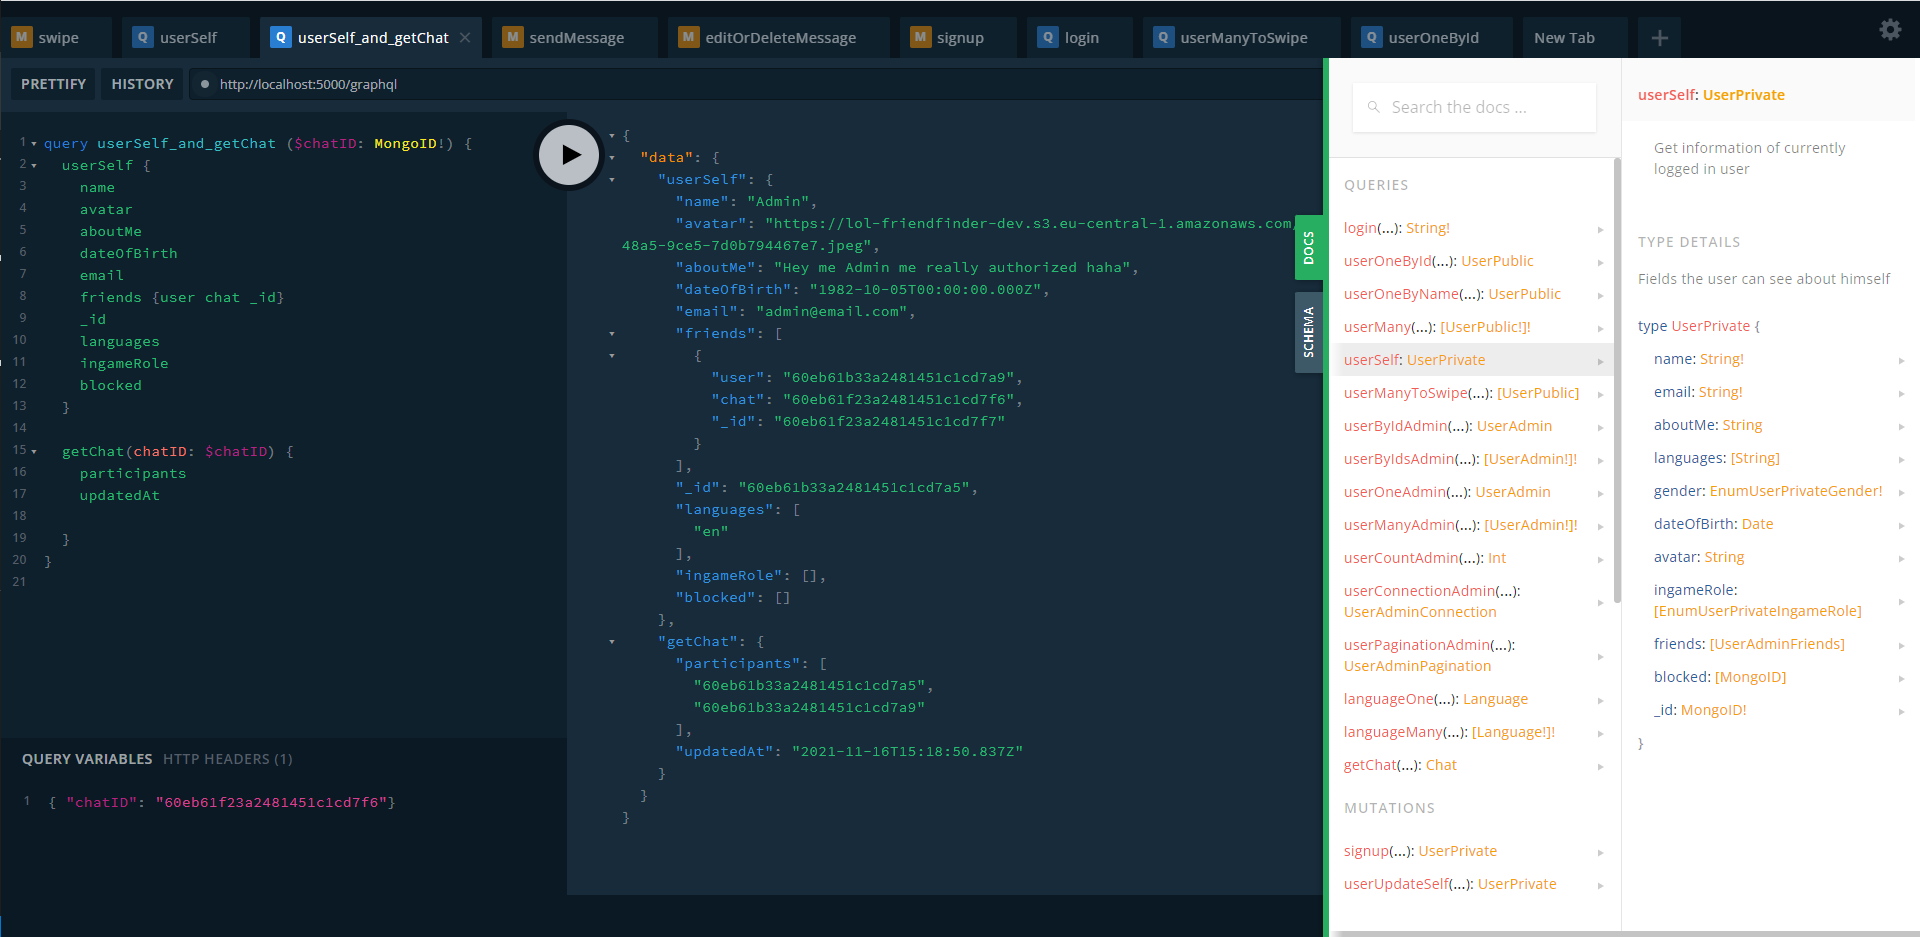
\includegraphics[width=\textwidth]{sources/graphiql.png}\cite{}
	\caption{GraphiQL Benutzeroberfläche. Links: Zwei Endpunkte werden durch eine Abfrage gebündelt abgefragt. Mitte: Antwort der Endpunkte. Rechts: Dokumentation und Typendefinition des Endpunkts \textit{userSelf}.}
	\label{figGQL1}
\end{figure}

\subsection{Resolver}
Durch die Pakete \textit{graphql-compose} und \textit{graphql-compose-mongoose} werden aus den bestehenden Datenbankmodellen Typenschemata entsprechend der Datentypen erstellt, die in GraphQL weiterverwendet werden können. 
Resolver ("to resolve", etw. auflösen/abwickeln/klären) beantworten Abfragen und Mutationen.
Sie bilden das Bindeglied zwischen Schnittstellenabfrage und Datenbankantwort.
So wird beispielsweise eine Schnittstellenabfrage, welche nach dem Namen, Alter und Freitext des Nutzers "Foobar" fragt, durch einen Resolver in die entsprechende Datenbankabfrage übersetzt und die Antwort der Datenbank wiederum so editiert, dass diese der gewünschten Datenstruktur der Abfrage entspricht. %TODO schaubild stattdessen
Simplere Resolver, welche zum Beispiel einen einzelnen Datenbankeintrag durch die ID identifizieren (\textit{findOne}) oder anhand der bestehenden Datenstruktur einen Datenbankeintrag erstellen (\textit{createOne}), werden durch die verwendeten Pakete bereit gestellt und lassen sich in das Projekt integrieren.
Für komplexere Resolver lassen sich bestehende Resolver anpassen oder gänzlich neue erstellen.
Die verwendeten Resolver und Typenschemata werden dem \textit{schemaComposer} bereit gestellt, welcher aus den bestehenden Daten die Dokumentation generiert.


\subsection{Verwendete Abfragen und Mutationen}
\paragraph{}
Nachfolgend werden einige der verwendeten Abfragen und Mutationen exemplarisch vorgestellt.

\paragraph{}
Für den Registrierungsvorgang wird die Mutation \textit{signup} verwendet.
Durch die Angabe von Email, gewünschtem Namen und Passwort wird ein Nutzerkonto erstellt.
In Zukunft kann durch Angabe von Namen und Passwort mit der \textit{login} Abfrage ein Authentifizierungstoken erstellt werden.
Das Token wird bei Abfragen, die eine Authentifizierung oder Authorisierung verlangen, verwendet

\begin{figure}
	\centering
    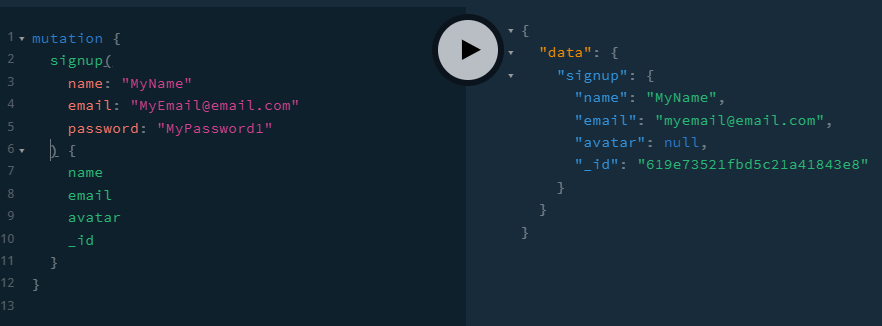
\includegraphics[width=\textwidth]{sources/graphiql_signup.png}\cite{}
	\caption{Registrierung des neuen Nutzers \textit{MyName}}
	\label{figGQL2}
\end{figure}

\begin{figure}
	\centering
    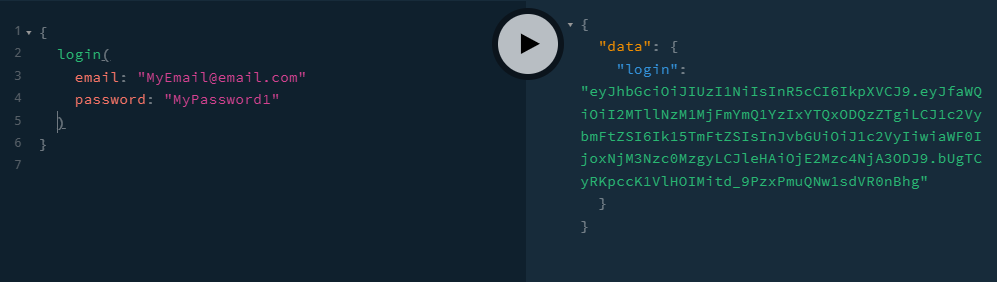
\includegraphics[width=\textwidth]{sources/graphiql_login.png}\cite{}
	\caption{Anmeldung des Nutzers. Die Antwort enthält das JSON Web Token, welches für bestimmte Abfragen zur Authentifizierung und Autorisierung dient.}
	\label{figGQL3}
\end{figure}

\paragraph{}
Alle weiteren vorgestellten Endpunkte benötigen zur eindeutigen Indentifizierung ein valides Authentifizierungstoken.

\paragraph{}
Um das eigene Profil anzuzeigen, wird die \textit{userSelf} Abfrage verwendet.
Diese zeigt Daten entsprechend des Datenbankschemas an.
Einige dieser Daten sind veränderbar, so zum Beispiel der Freitext.
Zum Verändern der Daten ist die Mutation \textit{userUpdateSelf} vonnöten.

\begin{figure}
	\centering
    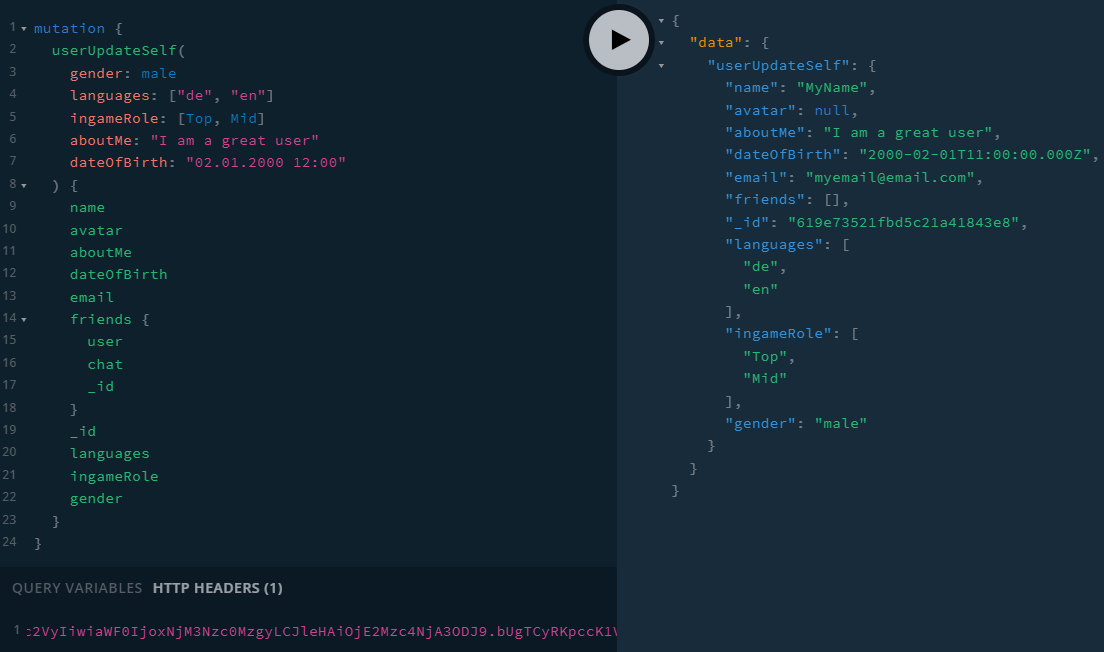
\includegraphics[width=\textwidth]{sources/graphiql_userUpdateSelf.png}\cite{}
	\caption{Das Geschlecht, Sprachen, Rolle etc. für den aktiven Nuter werden gesetzt. Unten: Ausschnitt des Autorisierungstokens. Durch das Token wird der aktive Nutzer identifiziert.}
	\label{figGQL4}
\end{figure}

Zum Finden von neuen Nutzern wird die Abfrage \textit{userManyToSwipe} verwendet. Dabei werden dem abfragendem Nutzer durch einen Algorithmus die Profile von mehreren Nutzern geladen, die sich nicht bereits in der Freundesliste befinden oder vom aktiven Nutzer blockiert wurden.
Nutzer, welche dem aktiven Nutzer eine Freundesanfrage geschickt haben, werden präferiert gezeigt, um die Chance neuer Freundschaften zu erhöhen.
Es ist möglich, durch Filter die Menge der potenziellen Nuter zu reduzieren.
Im Frontend werden die Profile nacheinander angezeigt.
Es wäre möglich gewesen,  mit jeder Abfrage nur einen einzelnen Nutzer anzuzeigen.
Da das Laden von mehreren Nutzern pro Abfrage jedoch die Zahl der Abfragen stark erhöht, wurde sich dagegen entschieden.
Mit der Mutation \textit{swipe} kann dann eine Freundschaftsanfrage an den angegebenen Nutzer geschickt werden.

\begin{figure}
	\centering
    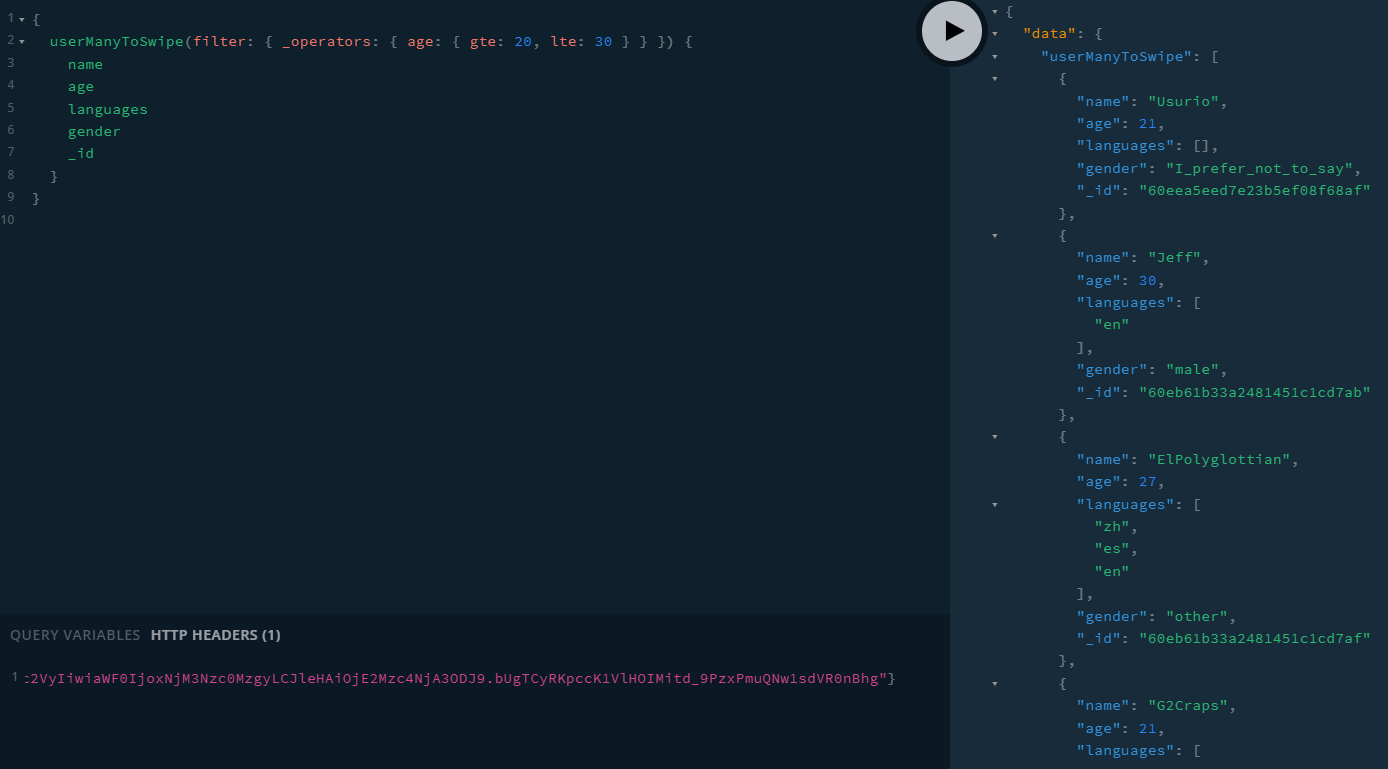
\includegraphics[width=\textwidth]{sources/graphiql_userManyToSwipe.png}\cite{}
	\caption{Abfrage nach mehreren Nutzern mit userManyToSwipe. Durch den Filter werden nur Nutzer im Alter zwischen 20 und 30 Jahren angezeigt.}
	\label{figGQL5}
\end{figure}

\begin{figure}
	\centering
    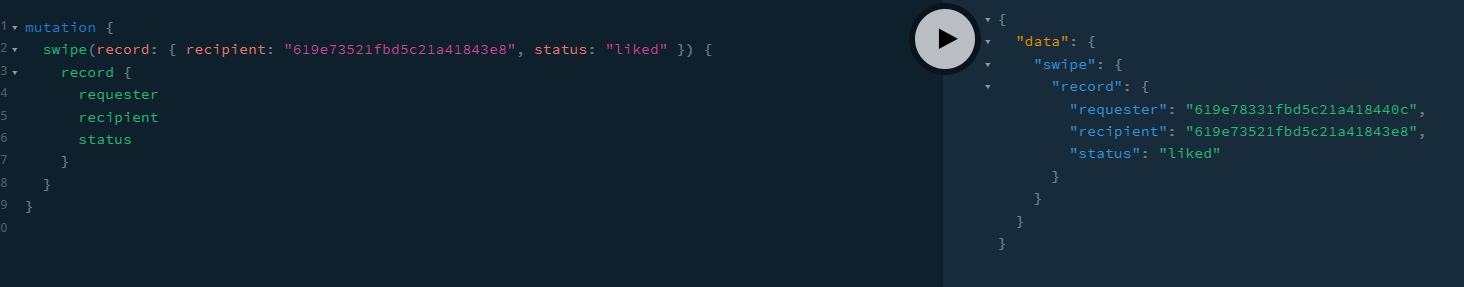
\includegraphics[width=\textwidth]{sources/graphiql_swipe.png}\cite{}
	\caption{Der aktive Nutzer versendet einen Like an den durch \textit{recipient} definierten Nutzer}
	\label{figGQL6}
\end{figure}

Die Nachrichten eines Chats können durch die Abfrage \textit{getChat} gelesen werden.
Dazu ist die ID des Chat anzugeben.
Der optionale Parameter "Seite" gibt an, welche Nachrichten zurückgegeben werden sollen.
Auf jeder Seite befinden sich 20 Nachrichten, beginnend bei \enquote{Seite=1} mit den neuesten 20 Nachrichten.
Sollte der Seitenparameter nicht angegeben werden, wird nur die neueste Nachricht geladen.
Dies wird bei der Vorschau des Chats für die Freundesliste verwendet.

\begin{figure}
	\centering
    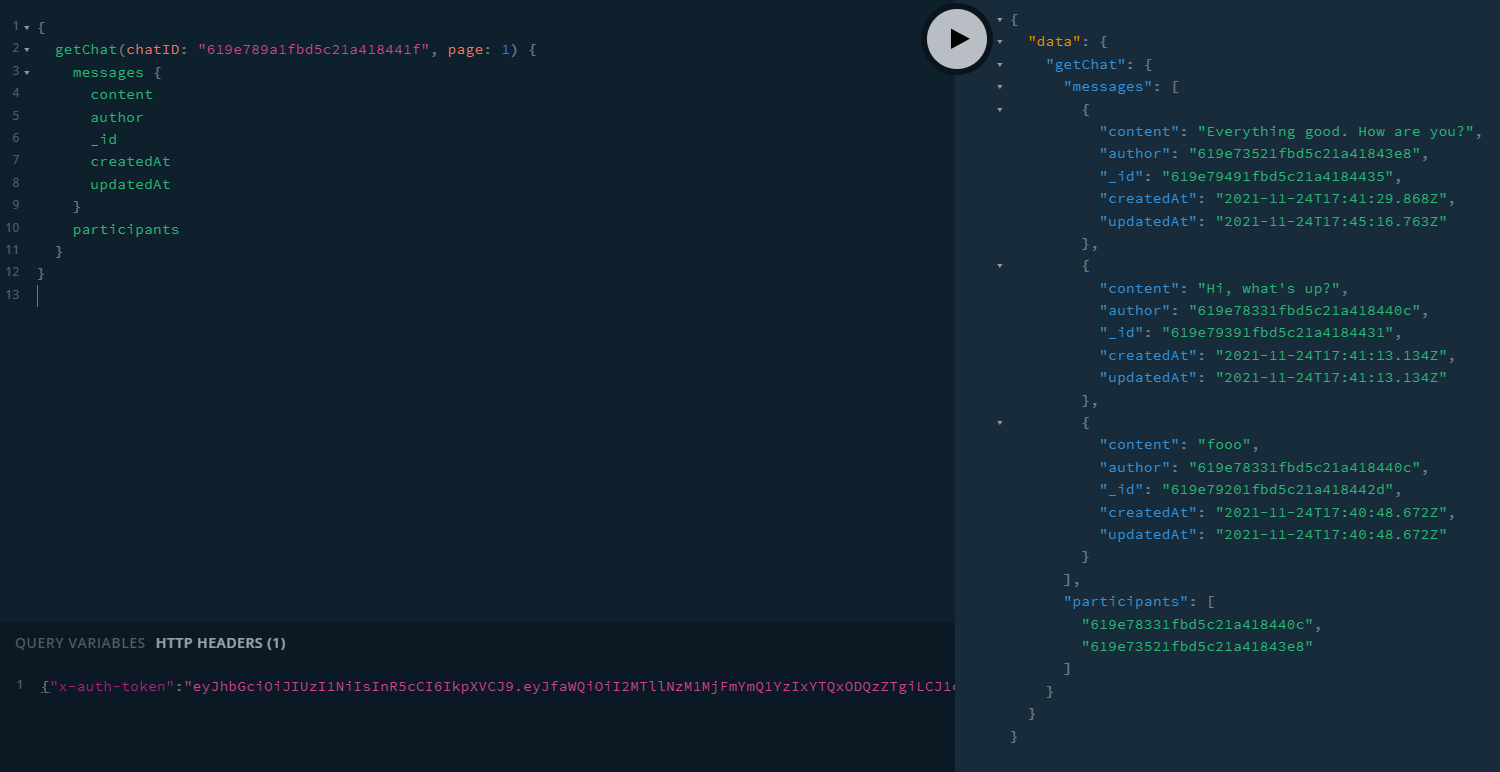
\includegraphics[width=\textwidth]{sources/graphiql_getChat.png}\cite{}
	\caption{Durch den Parameter \textit{page: 1} werden die bis zu 20 letzten Nachrichten geladen. Da der Chat nur 4 Nachrichten beinhaltet werden nur diese geladen. Unten: Das Authentifizierungstoken \textit{x-auth-token} befindet sich in dem HTTP-Header der Abfrage.}
	\label{figGQL7}
\end{figure}

Mit \textit{sendMessage} können Nachrichten versendet werden. Dazu ist die ID des Chats notwendig.
Der im Parameter \textit{Inhalt} definierte Text wird dann in den Chat als neueste Nachricht versendet.
Um eine Nachricht zu editieren  oder zu löschen, ist die Mutation \textit{editOrDeleteMessage} zu verwenden.
Zusätzlich zur Chat-ID ist die Nachrichten-ID der zu verändernden Nachricht anzugeben. Der optionale Parameter \textit{content} gibt im Falle einer Änderung den neuen Nachrichteninhalt an.
Sollte \textit{content} nicht definiert sein, wird die gewählte Nachricht stattdessen gelöscht. 

\begin{figure}
	\centering
    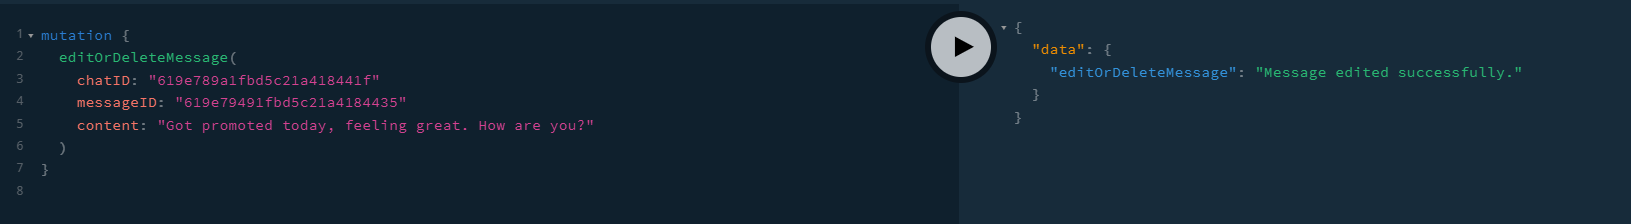
\includegraphics[width=\textwidth]{sources/graphiql_editMessage.png}\cite{}
	\caption{Die bestehende Nachricht (Siehe Abfrage \textit{getChat}) wird durch den in \textit{content} definierten Text ersetzt.}
	\label{figGQL8}
\end{figure}

\begin{figure}
	\centering
    \includegraphics[width=\textwidth]{sources/graphiql_deleteMessage.png}\cite{}
	\caption{Die soeben editierte Nachricht wird gelöscht.}
	\label{figGQL9}
\end{figure}

\subsection{Fazit}
Mit Hilfe von GraphQL konnten Endpunkte für Abfragen geschaffen werden, welche sich auf der Webseite unter der Benutzeroberfläche befinden. ... % TODO Fazit

\newpage
\section{Frontend}\label{kap_Frontend}
%\subsection{Wahl der Frontendtechnologie}
Das Frontend ist für die Datenvisualisierung zuständig und erleichtert dem Endbenutzer die Datenmanipulation. In diesem Kapitel werden \textit{Angular} und \textit{React} für die Entwicklung des Frontends bewertet. Beide Technologien haben unter anderem die Vorteile, gut dokumentiert zu sein und große Entwicklergemeinschaften zu haben\cite{SO01}. Dies begünstigt den Lernprozess und beschleunigt mögliche Problembehebungen. Große Entwicklergemeinschaften, bestehend aus Einzelpersonen und Unternehmen entwickeln die Frameworks weiter, wobei Angular von \textit{Google} und React von \textit{Meta (ehemals Facebook)} betreut wird. Die Technologien sind komponentenbasiert, was ihre Testbarkeit erleichtert. Maßgeblich an der Wahl der Technologien zum Vergleich verantwortlich war ihre Popularität - sie belegen in diversen Ranglisten die ersten Plätze\cite{SO01}.
\\\\
Folgende Kriterien werden berücksichtigt:
\begin{itemize}
  \item
         Der Schwierigkeitsgrad, um die Technologie zu lernen: Eine einfachere Technologie erlaubt es, früher mit der Durchführung des Projektes anzufangen und spart so Zeit und Kosten und damit das finanzielle Risiko.
  \item
        Die Akzeptanz bei den Entwicklern und die Anzahl von heruntergeladenen \textit{NPM-Paketen}. Vermehrte Nutzung von Paketen erhöht die Wahrscheinlichkeit, dass Probleme in diesen schnell identifiziert und gelöst werden\cite{LIN1}.
  \item
        Vorkenntnisse des Entwicklungsteams.
        %\item
        % Die Flexibilität des Frameworks.
        % Der Zwang, Probleme auf eine bestimmte Weise zu lösen, oder die Alternative, eigene Lösungswege zu finden.

        %  \item
        %  Anzahl der ungelösten Probleme\footnote{Open issues}.
\end{itemize}

\subsection*{Angular}
Angular ist ein Framework für Mobil- und Webanwendungen.
%STIMMT DAS? Angular lässt weniger Spielraum für eigene Entscheidungen darüber, wie der Code entwickelt wird. Deshalb eignet sich Angular besser für Projekte, wo mehrere Entwickler zusammenarbeiten.%Der Code wird mit Angular nach der Ri in einer vorgegebenen Art geschrieben werden sollte, um Einheitlichkeit zu schaffen.
Zu beachten ist, dass Angular nicht JavaScript als Hauptprogrammiersprache verwendet, sondern \textit{TypeScript}.
TypeScript ist ein striktes Superset von ECMAScript 2015.
TypeScript muss erstmal kompiliert werden, um auf dem Browser laufen zu können{\cite{MS1}}. Dieses Framework ist besonders geeignet für fortgeschrittene, umfangreiche Projekte.\footnote{{\citetitle*{AN1}}, Seite 30 \cite{AN1}}
%CHECK THIS
%https://merehead.com/blog/angular-vs-react-vs-vue-best-choice-2022/

\subsection*{React}
React ist eine Frontend-Technologie für die Entwicklung von Benutzeroberflächen für das Web und mobile Endgeräte\cite{GH08}.\footnote{Mithilfe von React-Native} React benutzt \textit{JSX}, welche eine HTML-ähnliche Syntax hat. Es wird von React empfohlen Komponenten mit JSX zu schreiben\cite{JSX1}. 
%Es besteht jedoch die Möglichkeit, diese in reinem JavaScript zu schreiben\cite{JSX1}.
\\
JSX ist eine JavaScript-Erweiterung. Diese bietet die Möglichkeit Code zu schreiben, der einfach zu lesen und zu schreiben ist. Die Verwendung von JSX hat unter anderem den Vorteil, \textit{XSS-Angriffe} zu verhindern.\footnote{Cross Site Scripting{\cite{OWASP}}} \cite{JSX1} Bei XSS-Angriffen es sich um eine Art von Sicherheitslücke, die in einigen Webanwendungen gefunden werden kann. Sie ermöglichen es Angreifern, clientseitige Skripte in Webseiten zu injizieren, die von anderen Benutzern aufgerufen werden. Für die Verwendung von JSX ist ein Compiler erforderlich, der den JSX-Code in reines JavaScript umwandelt.\footnote{\citetitle*{E01}, Seite 33 \cite{E01}}
%\\\\
%Laut einer StackOverFlow Umfrage hat React.js im Jahr 2021 jQuery als das am häufigsten verwendete Web-Framework überholt. {\cite{SO01}}
%Die Entwicklung mit Angular hätte mehr Zeit und Lernaufwand gekostet. Außerdem ist das Projekt nicht komplex genug, um das Angular-Ökosystem zu benötigen.

\subsection{Lernkurve}
Im Vergleich zu React ist Angular komplex und hat eine steile Lernkurve {\cite{E01}}.
\begin{quote}
  „Beispielsweise werden je nach Entwicklungsart bis zu fünf Dateien für eine einzelne Komponente benötigt, es müssen Abhängigkeiten eingefügt und die Komponenten in Modulen hinzugefügt werden. Infolgedessen wird ein Großteil der Entwicklungs-zeit in Angular für sich wiederholende Aufgaben aufgewendet.”
  {\citetitle*{AN1}, Seite 33\cite{AN1}}
\end{quote}
Der Lernaufwand und die Entwicklung mit Angular beansprucht daher mehr Zeit, als die mit React.

\subsection{Popularität}
Die unten aufgeführten Indikatoren sind wichtig, denn je mehr Menschen an einem Open-Source-Projekt beteiligt sind, desto mehr Menschen tragen dazu bei, Fragen zu beantworten und Probleme beim Quellcode zu lösen {\cite{LIN1}}.
\\
Im folgenden wird die Beliebtheit und die Nutzung von React und Angular anhand von verschiedenen Metriken betrachtet.
\\\\
\subsubsection*{Developer Survey 2021 - StackOverFlow}
\textit{StackOverFlow} ist eine Gemeinschaft von Softwareentwicklern, wo Wissen und Fragen zur Softwareentwicklung ausgetauscht werden. Seit 2011 führt StackOverFlow eine jährliche Umfrage zur Softwareentwicklung durch.
Die \autoref{fig:Most_popular_Web_Frameworks_2021} zeigt die Ergebnisse einer der Fragen. \\
Die Frage lautet, mit welchem Framework und welcher Bibliothek im letzten Jahr gearbeitet wurde und mit welcher im nächsten Jahr gearbeitet werden möchte. Auf der linken Seite stehen die prozentualen Ergebnisse und auf der rechten Seite die Anzahl der Antworten. Von den 67.593 Befragten waren 49.941 professionelle Entwickler. 
  
  \begin{figure}[h!]
    \centering
    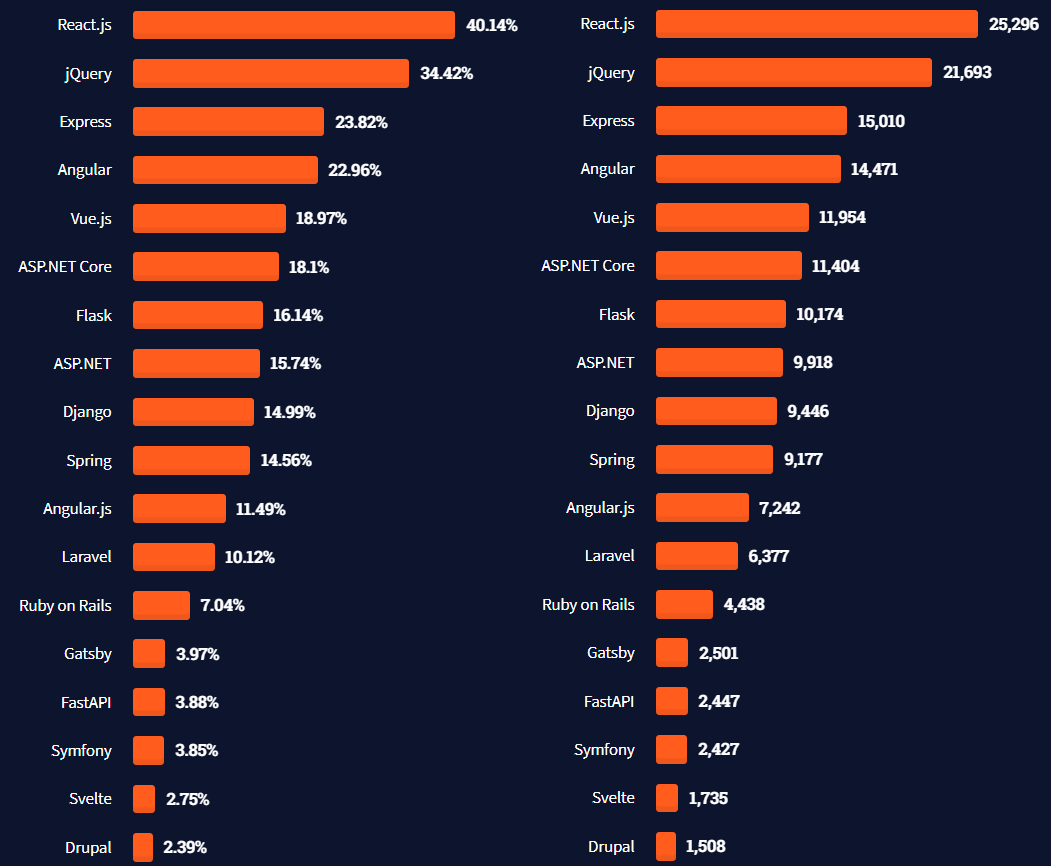
\includegraphics[scale=0.5]{sources/Most_popular_Web_Frameworks_2021}
    \caption[Most popular Web Frameworks 2021]{}
    \label{fig:Most_popular_Web_Frameworks_2021} 
    Ergebnisse der Umfrage: "Welche Frameworks und Bibliotheken haben Sie im letzten Jahr stark genutzt?" (links) und "Wollen Sie diese im nächsten Jahr verwenden?" (rechts) (Mehrfachnennungen möglich)\cite{SO01}.
  \end{figure}

\subsubsection*{Github}
\textit{GitHub} ist eine Plattform für die Versionskontrolle von Source-Code, auf der mehr als 238 Millionen Repositories verwaltet werden{\cite{GH07}}.
Die Anzahl der Repositories, in denen Code für Angular und React gespeichert wird, gibt einen Hinweis auf die Beliebtheit dieser Frameworks.
\\
\begin{table}[h!]
  \centering
  \begin{tabular}{ |p{5cm}||p{3.6cm}|p{3.6cm}|  }
    \hline
    \multicolumn{3}{|c|}{Github Statistiken}\\
    \hline
    & Angular/core  {\cite{GH04}}& React {\cite{GH06}}\\
    \hline
    Anzahl von Repositories & 2,011,663& 7,868,546
   % \\
    %\hline
    %Sterne & 77.2k & 170k
    \\
    \hline
  \end{tabular}
\end{table}

%https://risingstars.js.org/2020/es#section-statemanagement
%https://www.freecodecamp.org/news/angular-react-vue/
%Sterne sind eine von GitHub verwendete Metrik, um die Beliebtheit von Repositories auf GitHub zu messen.
\newpage
\subsubsection*{Node Package Manager (NPM)}
\textit{NPM} ist ein Repository für die Veröffentlichung von Open-Source-Node.js-Projekten. Mithilfe von NPM werden auch die Abhängigkeiten eines Angular oder React Projekts verwaltet. Die Anzahl der heruntergeladenen NPM-Pakete gibt einen Hinweis auf die Nutzung der Technologie.
\begin{figure}[h!]
  \centering
  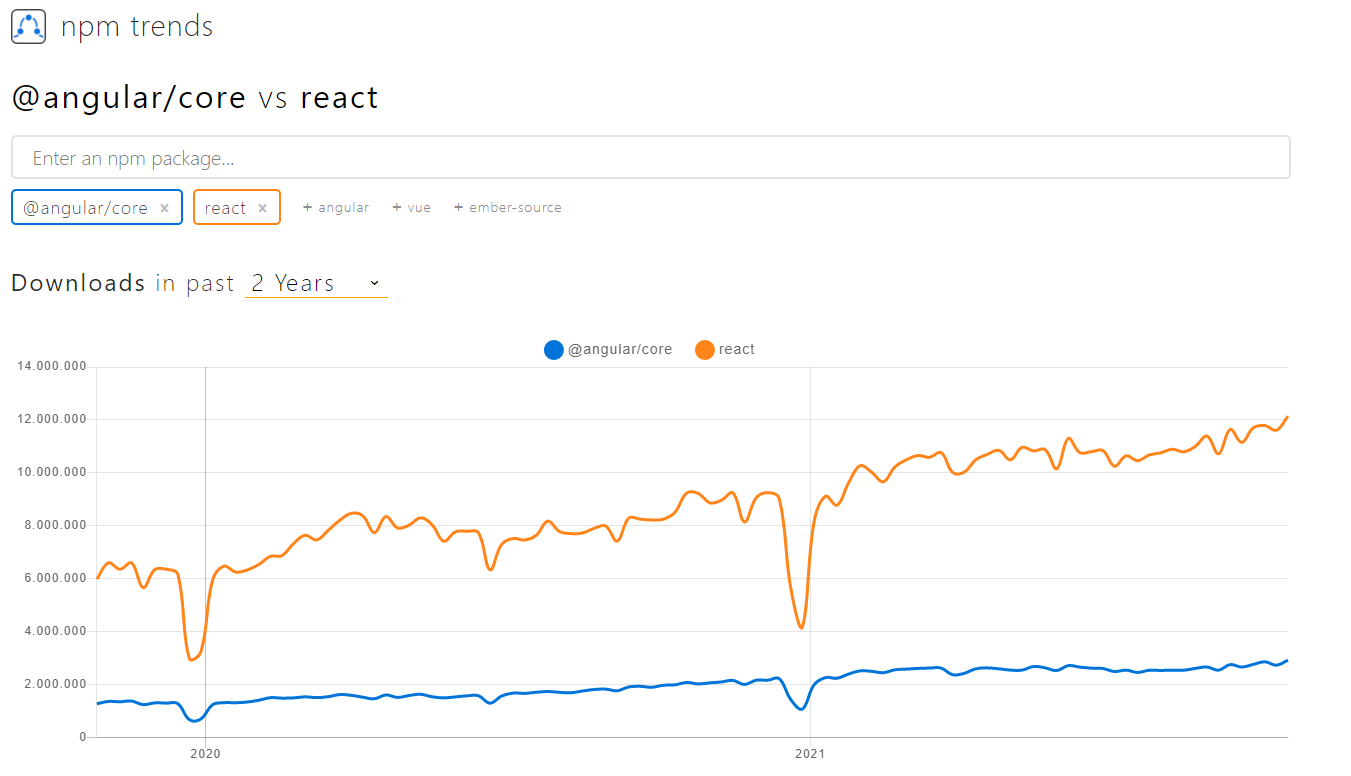
\includegraphics[scale=0.4]{sources/NPM-Trends React_Angular}
  \caption[Heruntergeladene NPM-Pakete]{}
  \label{fig:NPM-Trends React_Angular} 
  Heruntergeladene NPM-Pakete @angular/core vs react
   {\cite{NPM01}}
\end{figure}


\subsubsection*{Google Trends}
\textit{Google Trends} ist ein Werkzeug, mit dem die Entwicklung der Anzahl der Suchanfragen für ein bestimmtes Stichwort oder Thema im Laufe der Zeit verfolgt wird\cite{GO02}. In Zeitraum zwischen 01.11.2020 und 26.10.2021 wurde nach React häufiger als nach Angular gesucht. Dies belegen die Daten von Google Trends in der \autoref{fig:GoogleTrends React Angular 1.11.2020 29.10.2021}. Diese Metrik ist ein weiterer Beweis für die Beliebtheit des Frameworks.

\begin{figure}[h!]
  \centering
  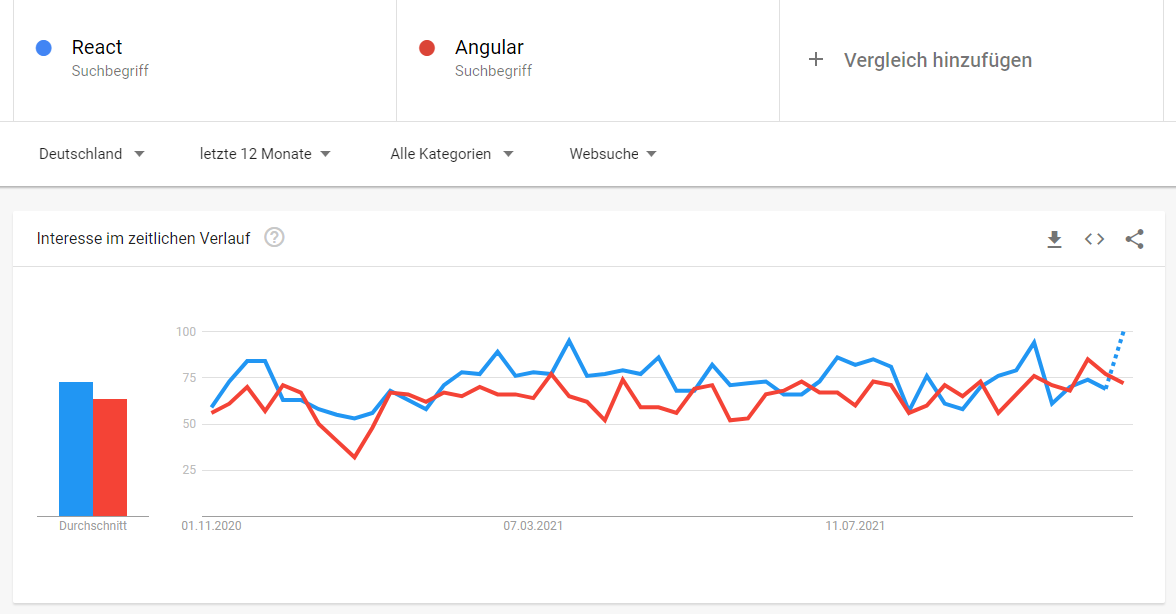
\includegraphics[scale=0.5]{sources/GoogleTrends React Angular 1.11.2020 29.10.2021}
  \caption[Google Trends Angular vs React]{}
  \label{fig:GoogleTrends React Angular 1.11.2020 29.10.2021} 
  Google Trends Angular vs React{\cite{GO01}}.
\end{figure}

\subsubsection*{Jobangebote}
Als angehende Informatiker sind berufliche Perspektiven relevant für unterstützt, deswegen wurde der Arbeitsmarkt in der Entscheidungsfindung berücksichtigt.
\\
  %In der Entscheidungsfindung sind ebenfalls künftige Perspektiven relevant.
  %Aus diesem Grund ist als angehende Informatiker den Arbeitsmarkt berücksichtigt.   
Anzahl der Jobangebote bei \textit{LinkedIn} in Deutschland:\\
Angular: 7.657 Ergebnisse{\cite{LI1}}\\
React: 11.523 Ergebnisse{\cite{LI2}}

\subsection{Vorkenntnisse}
Das Entwicklungsteam verfügt über Javascript-Kenntnisse, was für die Wahl einer Technologie wie React spricht, die keine neuen Kenntnisse erfordert. Durch das vorhandene Wissen wird die Entwicklungszeit beschleunigt und mögliche Weiterbildungskosten vermieden.

\subsection{React Hooks}
%https://www.javatpoint.com/react-hooks
Beginnend mit der Version 16.8.0, enthält React eine stabile Implementierung von React Hooks. Ab dieser Version wird von React empfohlen, keine Klassen mehr für die Erstellung von Komponenten zu verwenden\cite{R01}. Mit Klassen geschriebene Komponenten werden weiterhin unterstützt und müssen nicht neu geschrieben werden{\cite{R05}}. Die \textit{Hooks} bieten eine leistungsstarke und ausdrucksstarke neue Möglichkeit zur Wiederverwendung von Funktionen zwischen Komponenten. Die Hooks sind ein direkterer Weg zur Nutzung der React-Funktionen im Vergleich zu Klassen. In diesem Projekt wurde \textit{useState} verwendet, um den Zustand der Applikation zu verwalten, \textit{useEffect} um das \textit{Rendering} von Informationen in der Benutzeroberfläche zu steuern und useContext, um die Applikationsinformationen zwischen den Komponenten zu verteilen.\footnote{In diesem Kontext ist Rendering die Darstellung von Inhalten in einer Benutzeroberfläche gemeint.}

\subsubsection*{useState}
Der Hook useState bietet die Möglichkeit an, den Zustand einer Anwendung zu verwalten. In diesem Projekt wurde useState verwendet, um alle Benutzerdaten zu manipulieren und lokal zwischen zu speichern. Nachdem der Client eine gültige Abfrage an den Server gesendet hat, werden die Daten in den durch useState definierten Variablen gespeichert.
\begin{figure}[h!]
  \centering
  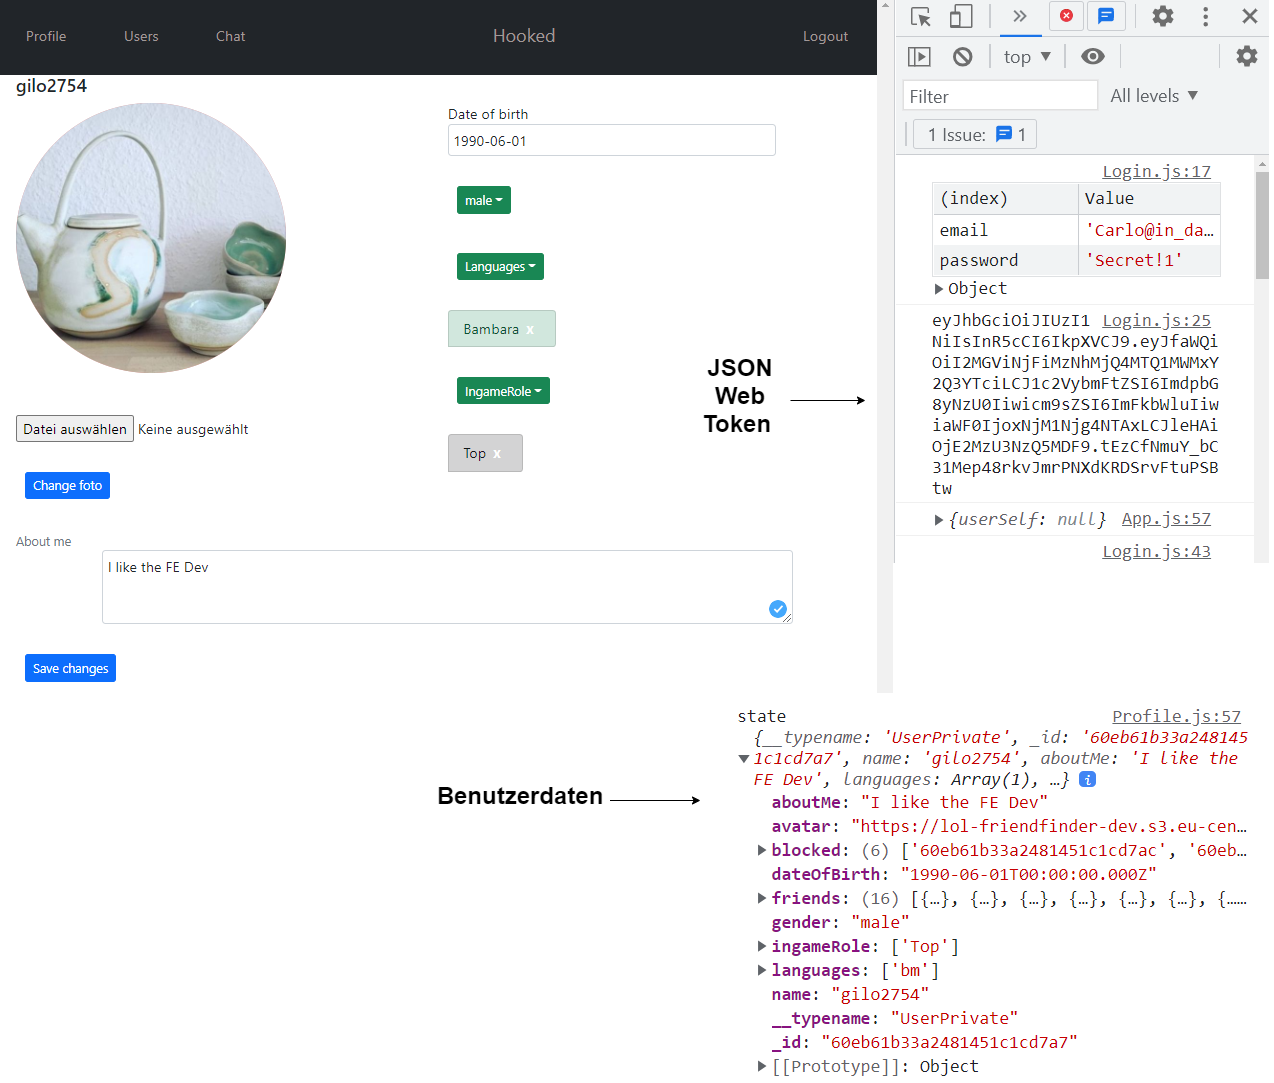
\includegraphics[scale=0.35]{sources/Server-Abfrage-Antwort}
  \caption{Antwort einer Serverabfrage. Eigene Darstellung.}
  \label{fig:Antwort_Serverabfrage} 
  %\cite{AMZ20}
\end{figure}
Die \autoref{fig:Antwort_Serverabfrage} zeigt eine Abfrage an den Server für die Anmeldung, diese gibt das JSON Web Token zurück, welches die Aufrechterhaltung einer aktiven Sitzung ermöglicht.\footnote{Authentifizierungstoken\cite{be:rfc7519}} Dieses Token wird für künftige Abfragen benötigt, um den Zugriff auf die Informationen des Nutzers zu ermöglichen.\footnote{Eine genauere Funktionsweise der Serverabfragen folgt in Kapitel~\ref{kap_Schnittstelle}.}
%In späteren Kapiteln wird näher erläutert, wie diese Informationen, die durch einen einzigen Abfrage an den Server erhalten werden, in den Chat- und Benutzerkomponenten genutzt werden.
%Wie man sieht, gibt es innerhalb des states nicht nur einen Wert, sondern mehrere.
%Es handelt sich eigentlich um ein Objekt. Objekte sind dasselbe wie Variablen in JavaScript, der einzige Unterschied ist, dass ein Objekt mehrere Werte in Form von Eigenschaften und Methoden enthält.
%Objekte können andere Objekte, Strings, Arrays, Zahlen und so weiter enthalten.
%\newpage
\subsubsection*{useEffect}
\textit{useEffect} ermöglicht es, verschiedene Arten von Effekten zu erzeugen, nachdem eine Komponente gerendert wurde. Unter Effekten versteht man die Art und Weise, in der Daten angezeigt werden. useEffect kümmert sich um die Aktualisierung des HTML-DOM, wenn dies erforderlich ist.\footnote{Document Object Model {\cite{MO2}}} Die Aktualisierung des HTML-DOM erfolgt auf Komponentenebene. Nur die Komponenten, die aktualisiert werden müssen, werden neu geladen.\\
Dies ist möglich, indem  das virtuelle React-DOM und das HTML-DOM im Browser verglichen werden\cite{R06}.\footnote{{\citetitle*{AN1}, Seite 22 \cite{AN1}}} Wenn der Benutzer Änderungen im Bereich Benutzerprofil vornimmt, werden diese erstmal in der Variable „state” zwischengespeichert, bevor sie in der Datenbank gespeichert werden. Die Abfrage zur Aktualisierung der Daten wird in dem Moment an den Server gesendet, in dem der Benutzer auf die Taste „Save“ drückt. Zu diesem Zeitpunkt wird die Benutzeroberfläche durch useEffect aktualisiert, da die Variable „state” als Abhängigkeit von useEffect festgelegt ist und diese neue Informationen enthalten.
\\\\
Ein Beispiel dafür ist, wenn der Benutzer das Feld Sprachen aktualisiert. Beim Speichern der Änderungen werden nur die Komponenten der vorgenommenen Änderung zusammenhängt, wieder in das HTML-DOM geladen.

\subsubsection*{useContext}
\textit{useContext} ermöglicht Daten innerhalb bestimmter Komponenten zu teilen. In diesem Projekt wird useContext eingesetzt, um die Benutzerdaten und den Authentifizierungstoken über die Komponenten  „Profile“, „Chat“ und „Users“ zu teilen. UseContext bietet eine Lösung, um Daten zwischen Komponenten auszutauschen{\cite{R04}}.
\newpage
In diesem Projekt war es nötig, Daten über mehrere Komponenten zu teilen, weil die Benutzerdaten in mehreren Komponenten konsumiert wurden. Zum Beispiel, die Kennung\footnote{User id} der Freunde eines Benutzers, ist in der Variable „state” gespeichert. Diese Informationen werden in der Komponente „Chat” verwendet, um Einzelheiten über die Freunde des angemeldeten Benutzers bereitzustellen. Zusätzlich befindet sich auch in der Variable „state” die Kennung der Nachrichten pro Benutzer.\footnote{Chat id} Diese wurde verwendet, um die Nachrichten abzufragen, die von Benutzern untereinander ausgetauscht wurden. 
Die oben genannten Informationen zeigen die \autoref{fig:Friends_in_Chat}.
\begin{figure}[h!]
  \centering
  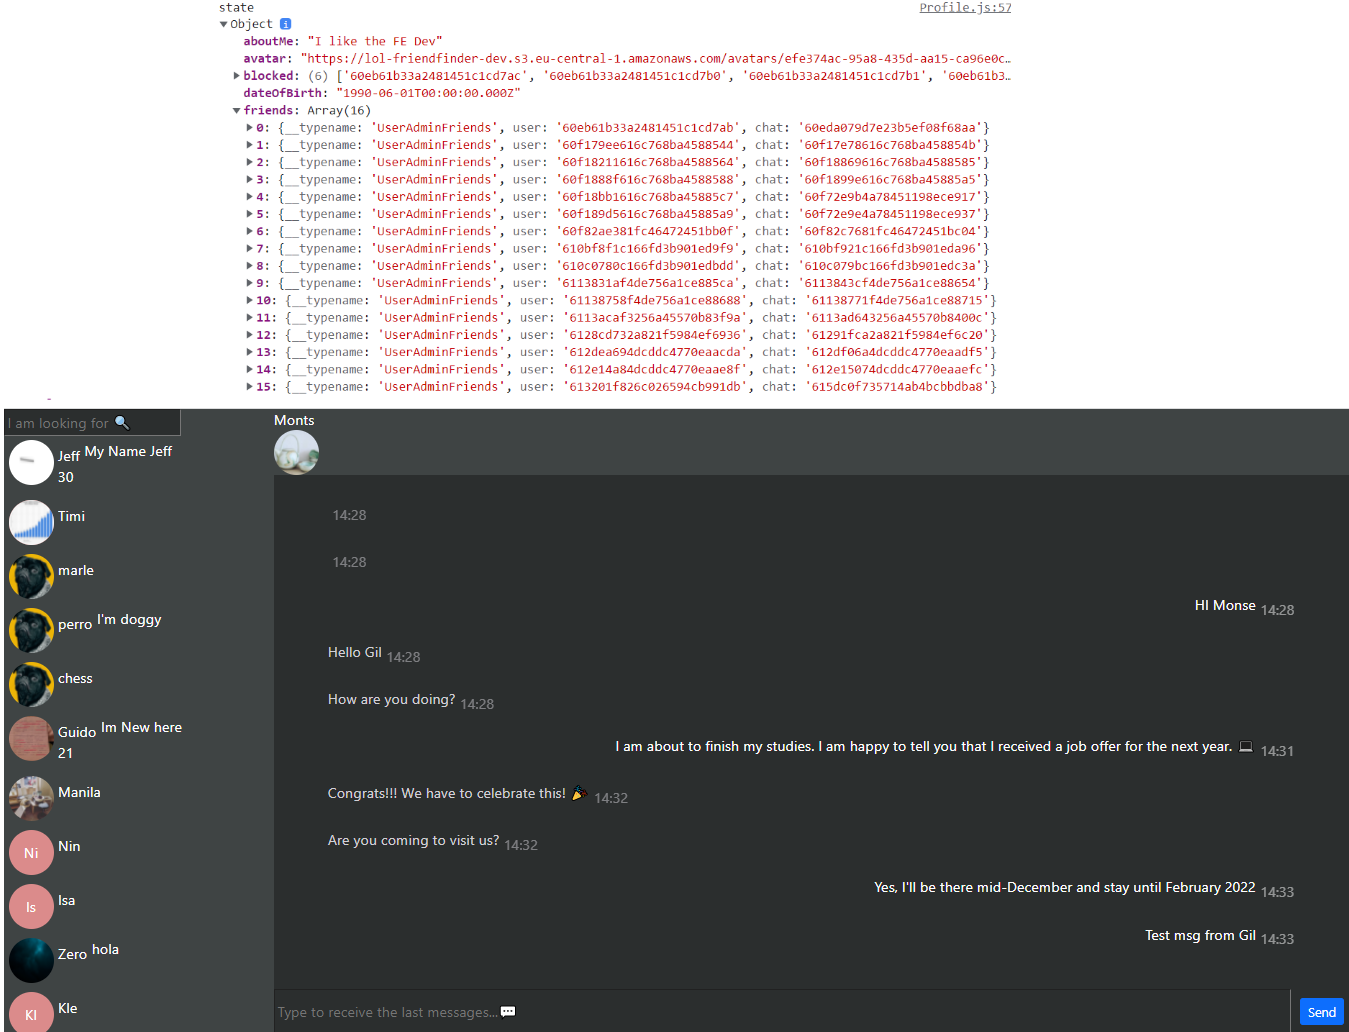
\includegraphics[scale=0.43]{sources/Friends_in_Chat}
  \caption[Einzelheiten der Freunde]{}
  \label{fig:Friends_in_Chat} 
  die grafische Ansicht des Chats und der Konsole. Eigene Darstellung.
\end{figure} 
%Im Anhang 5 und 6 befidet sich der Code mit dem den Authentifizierungstoken und die Benutzerdaten global  mithilfe von useContext verwaltet wird.
%subsection*{Fazit}
\newpage
Die \autoref{fig:Angular_vs_React} fasst die wichtigsten Unterschiede und Gemeinsamkeiten zwischen React und Angular zusammen.
\\
  \begin{figure}[h!]
    \centering
    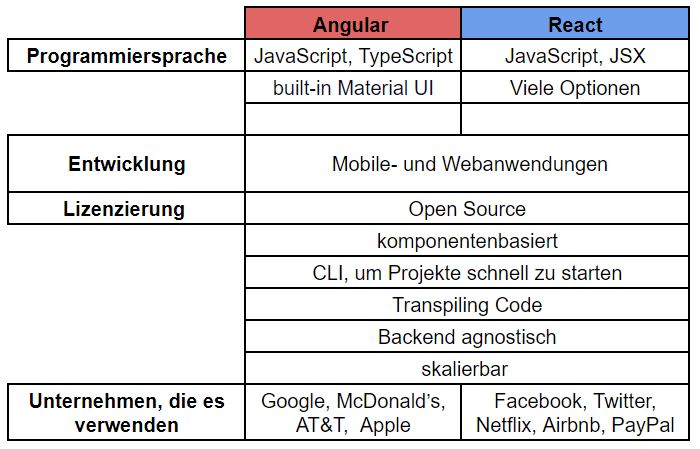
\includegraphics[scale=0.5]{sources/Angular_vs_React}
    \caption[Vergleich Angular vs React]{}
    \label{fig:Angular_vs_React} 
    Vergleich Angular vs React. Eigene Darstellung. Quelle:
    \cite{AvsR}, {\citetitle*{E01}, Kap.3 S.14-22 Kap.4 S.33\cite{E01}}
  \end{figure}
\\
   In diesem Kapitel wurde gezeigt, wie React für die Erstellung der Benutzeroberfläche verwendet wurde. Es ist anzumerken, dass die Entwicklung des Projekts mit jedem der beiden Frameworks möglich ist. Bei der endgültigen Entscheidung wurde React aufgrund einer geringen Lernkurve, guter Zustandsverwaltung, großer Popularität und Einfachheit gewählt.


\newpage
\section{Qualitätssicherung }\label{kap_QS}
\input{chapters/Qualitätssicherung}

\newpage
\section*{Zusammenfassung }\label{kap_ZF}
\addcontentsline{toc}{section}{Zusammenfassung}
%Es hat sich gezeigt, dass mit modernen JavaScript-Entwicklungswerkzeugen 
%auch ohne umfassende Kenntnisse der Softwareentwicklung zugänglich sind.
Es hat sich gezeigt, wie die Entwicklung einer Webanwendung nach dem MERN-Stack erfolgt. Dies in einem Zeitraum von Mai 2021 bis Mitte August 2021. Mit grundlegenden Programmierkenntnissen war es möglich, eine funktionelle Anwendung mit folgenden Funktionen zu entwicklen; die Registrierung für neue Benutzer, die Anmeldung für bestehende Benutzer, die Verwaltung deren persönlichen Daten, die Interaktion mit anderen Benutzern auf der Grundlage ihrer Präferenzen und einen auf Textnachrichten basierenden Kommunikationskanal.
\\\\
%TInfra
In Kapitel \ref{kap_Technologieinfrastruktur} wurde die Architektur der Anwendung kurz eingeführt. %DB
Die Auswahl der Datenbank und deren Schemata wurde in Kapitel \ref{kap_Datenbank} erläutert. In Kapitel \ref{kap_Backend} und \ref{kap_Schnittstelle} befindet sich die Logik, um die Daten der Datenbank zu manipulieren. An dieser Stelle wurde erklärt, wie die REST-Schnittstelle für das Profilbild im Amazon S3 und die GraphQL-Endpunkte für die Verwaltung der Nutzerdaten entwickelt wurde.  
%Backend %Schnittstelle 
%Frontend
Das Kapitel \ref{kap_Frontend} zeigt welche Kriterien für die Wahl von React berücksichtigt wurden. Außerdem, wurde die Entwicklung der Benutzeroberfläche mit React-Hooks gezeigt. 
%Qualitätssicherung
Die Erstellung von den Unit- und End-To-End-Tests beschrieben im Kapitel \ref{kap_QS} würde die Testzeit für komplexere Anwendungen beschleunigen. Im Falle des vorliegenden Projekts handelte es sich um ein zusätzlicher Werkzeug, dessen Einbindung in den Entwicklungszyklus etwa fünf Tage in Anspruch nahm. %Einer signifikante Wert haben die Unit-Test, 
%Was konnte nicht geschafft werden?
\\\\
Der Fokus lag daran, eine funktionelle Anwendung zu entwicklen. Es hat sich auf Funktionen verzichtet, welche die geplante Zeitraum des Projekts überschritten. Unter anderem die Anmeldung über SSO mit zum Beispiel eine Facebook- oder Google-Konto. %Für einen späteren Zeitpunkt wird sich dieses Projekt bei WIE HEISST DAS?
Eine bessere Gebrauchlichkeit %Usability 
bietet für die vorliegenden Applikation, eine mobile Applikation. Deshalb ist es sinnvoll eine weitere Version der Anwendung mit React-Native umzuwandeln.

%Glossar
%\newpage


% Anhang
\newpage
\section*{Anhang}\label{anhang}
\addcontentsline{toc}{section}{Anhang} % Manuellen Eintrag im Inhaltsverzeichnis erzeugen
\subsection{Aufwandsverteilung}\label{subsec_UabsAnhang}
Hier zeigen wir, wie die Aufgaben unter den Autoren des Projekts verteilt wurden.
TABELLE/Bild KOMMT...

\subsection{ANHAND X}\label{subsec_UabsAnhang}


\subsection{Verwendete Technologien und Werkzeuge}\label{subsec_UabsAnhang}
NodeJS
\\
React
\\
Bootstrap
\\
GitHub
\\
Cypress
\\
VSC
\\
Heroku
\\
LaTeX
\\
Cypress

%Bib
\newpage
\printbibliography[heading=bibintoc]

% Erklärung über die selbständige Abfassung der Arbeit
\pagestyle{empty}
\section*{Erklärung über die selbständige\\Abfassung der Arbeit} % \section*{...}: das *-Symbol erlaubt, dass dieser
% Gliederungspunkt nicht ins Inhaltsverzeichnis aufgenommen wird
\addcontentsline{toc}{section}{Erklärung über die selbständige Abfassung der Arbeit}
Ich versichere, die von mir vorgelegte Arbeit selbständig verfasst zu haben.
Alle Stellen, die wörtlich oder sinngemäß aus veröffentlichten oder nicht veröffentlichten Arbeiten anderer entnommen sind,
habe ich als entnommen kenntlich gemacht.\\
Sämtliche Quellen und Hilfsmittel, die ich für die Arbeit benutzt habe, sind
angegeben. Die Arbeit hat mit gleichem Inhalt bzw. in wesentlichen Teilen noch keiner anderen Prüfungsbehörde vorgelegen.\\\\
\begin{tabular}{cp{7cm}}
                                    &             \\
          Gummersbach                   &             \\ \hline
  \small (Ort, Datum, Unterschrift) & \normalsize \\
\end{tabular}


\newpage
% Unbeschriftetes Abschlussblatt (Leere Seite)
\thispagestyle{empty}
\input{leereSeite}

\end{document}

